% Options for packages loaded elsewhere
\PassOptionsToPackage{unicode}{hyperref}
\PassOptionsToPackage{hyphens}{url}
%
\documentclass[
]{article}
\usepackage{amsmath,amssymb}
\usepackage{lmodern}
\usepackage{iftex}
\ifPDFTeX
  \usepackage[T1]{fontenc}
  \usepackage[utf8]{inputenc}
  \usepackage{textcomp} % provide euro and other symbols
\else % if luatex or xetex
  \usepackage{unicode-math}
  \defaultfontfeatures{Scale=MatchLowercase}
  \defaultfontfeatures[\rmfamily]{Ligatures=TeX,Scale=1}
\fi
% Use upquote if available, for straight quotes in verbatim environments
\IfFileExists{upquote.sty}{\usepackage{upquote}}{}
\IfFileExists{microtype.sty}{% use microtype if available
  \usepackage[]{microtype}
  \UseMicrotypeSet[protrusion]{basicmath} % disable protrusion for tt fonts
}{}
\makeatletter
\@ifundefined{KOMAClassName}{% if non-KOMA class
  \IfFileExists{parskip.sty}{%
    \usepackage{parskip}
  }{% else
    \setlength{\parindent}{0pt}
    \setlength{\parskip}{6pt plus 2pt minus 1pt}}
}{% if KOMA class
  \KOMAoptions{parskip=half}}
\makeatother
\usepackage{xcolor}
\usepackage{longtable,booktabs,array}
\usepackage{calc} % for calculating minipage widths
% Correct order of tables after \paragraph or \subparagraph
\usepackage{etoolbox}
\makeatletter
\patchcmd\longtable{\par}{\if@noskipsec\mbox{}\fi\par}{}{}
\makeatother
% Allow footnotes in longtable head/foot
\IfFileExists{footnotehyper.sty}{\usepackage{footnotehyper}}{\usepackage{footnote}}
\makesavenoteenv{longtable}
\usepackage{graphicx}
\makeatletter
\def\maxwidth{\ifdim\Gin@nat@width>\linewidth\linewidth\else\Gin@nat@width\fi}
\def\maxheight{\ifdim\Gin@nat@height>\textheight\textheight\else\Gin@nat@height\fi}
\makeatother
% Scale images if necessary, so that they will not overflow the page
% margins by default, and it is still possible to overwrite the defaults
% using explicit options in \includegraphics[width, height, ...]{}
\setkeys{Gin}{width=\maxwidth,height=\maxheight,keepaspectratio}
% Set default figure placement to htbp
\makeatletter
\def\fps@figure{htbp}
\makeatother
\setlength{\emergencystretch}{3em} % prevent overfull lines
\providecommand{\tightlist}{%
  \setlength{\itemsep}{0pt}\setlength{\parskip}{0pt}}
\setcounter{secnumdepth}{-\maxdimen} % remove section numbering
\ifLuaTeX
  \usepackage{selnolig}  % disable illegal ligatures
\fi
\IfFileExists{bookmark.sty}{\usepackage{bookmark}}{\usepackage{hyperref}}
\IfFileExists{xurl.sty}{\usepackage{xurl}}{} % add URL line breaks if available
\urlstyle{same} % disable monospaced font for URLs
\hypersetup{
  hidelinks,
  pdfcreator={LaTeX via pandoc}}

\author{}
\date{}

\begin{document}

\textbf{NEUROSHELL: AN AI-ASSISTED PENETRATION TESTING
FRAMEWORKINDIVIDUAL THESIS}

HERATH H.M.C.H.K

IT22121592

Individual component: Dynamic Planner \& RAG Engine

Group ID: R26-CS-018

Report submitted in partial fulfilment of the requirements for the

Bachelor of Science Honours in Information Technology

Specialising in Cyber Security

Department of Computer System Engineering

Sri Lanka Institute of Information Technology

Sri Lanka

October 2026

DECLARATION AND SUPERVISOR CERTIFICATION

\textbf{Candidate declaration.} I declare that this thesis is my own
work and does not incorporate, without acknowledgement, material
previously submitted for a degree or diploma at any university or
institute of higher learning. To the best of my knowledge, it contains
no material previously published or written by another person except
where acknowledgement is made in the text. I grant the Sri Lanka
Institute of Information Technology the non-exclusive right to reproduce
and distribute this thesis, in whole or in part, in print, electronic,
or other media, while retaining the right to use the content in future
work.

\textbf{Academic integrity and AI disclosure.} I have disclosed all use
of generative AI and other automated tools in accordance with the module
policy. I remain responsible for the accuracy, originality, citations,
code, data, analyses, and conclusions in this thesis.

Student name: {[}Full name{]}

Student ID: {[}Student ID{]}

Signature: \_\_\_\_\_\_\_\_\_\_\_\_\_\_\_\_\_\_\_\_\_\_\_\_\_\_\_\_\_\_
Date: \_\_\_\_\_\_\_\_\_\_\_\_

\textbf{Supervisor certification.} The above candidate carried out this
research for the bachelor\textquotesingle s degree thesis under my
supervision.

\begin{longtable}[]{@{}
  >{\raggedright\arraybackslash}p{(\columnwidth - 4\tabcolsep) * \real{0.4483}}
  >{\raggedright\arraybackslash}p{(\columnwidth - 4\tabcolsep) * \real{0.3310}}
  >{\raggedright\arraybackslash}p{(\columnwidth - 4\tabcolsep) * \real{0.2207}}@{}}
\toprule()
\begin{minipage}[b]{\linewidth}\raggedright
\textbf{Role and name}
\end{minipage} & \begin{minipage}[b]{\linewidth}\raggedright
\textbf{Signature}
\end{minipage} & \begin{minipage}[b]{\linewidth}\raggedright
\textbf{Date}
\end{minipage} \\
\midrule()
\endhead
Supervisor: {[}Name{]} & & \\
Co-supervisor: {[}Name{]} & & \\
\bottomrule()
\end{longtable}

ABSTRACT

This research developed the Dynamic Planner and Retrieval-Augmented
Generation Engine as Component 2 of NeuroShell. The component converts
structured cybersecurity intents into commands for Nmap, Nikto, and
Gobuster. It combines intent interpretation, tool selection,
documentation retrieval, model-assisted command synthesis, and
validation before passing a planning response to the execution
component.

A Design Science Research approach guided the development and
evaluation. Command examples were prepared from a 9,391-record candidate
pool, with a final supervised dataset of 2,704 training, 338 validation,
and 337 test pairs. Direct evaluation compared the Gemma 2 2B
instruction model with its trained LoRA adapter enabled and disabled.
The adapted configuration achieved 295 exact matches out of 337
predictions, an exact-match rate of 87.54\%, and selected the requested
tool in every assessed prediction. Exact-match rates varied by tool:
67.26\% for Nmap, 98.28\% for Nikto, and 97.22\% for Gobuster. The base
configuration achieved no strict exact matches, a result influenced by
response formatting as well as command differences.

A separate 25-case base-model ablation recorded semantic command
accuracy of 56\% without retrieval and 84\% with retrieval. Average
planning latency increased from 12.03 to 21.75 seconds in that
experiment. The selected backend verification run passed all 42 tests,
covering API behaviour, command validation, safety filtering, intent
interpretation, and semantic evaluation. These experiments assess
different configurations and do not form a single end-to-end accuracy
result.

The contribution is an implemented planning service with explicit task
contracts, documentation grounding, and checks on generated commands.
The evidence supports its use as a bounded research prototype. Reference
inconsistencies, uneven task coverage, unmeasured final-model semantic
accuracy, and the absence of user trials limit broader conclusions.
Further work should improve dataset auditing, assess deployment parity,
and evaluate the complete authorised workflow.

Keywords: command synthesis, retrieval-augmented generation,
cybersecurity, structured intent, command validation

ACKNOWLEDGEMENTS

I would like to express my sincere thanks to my supervisor for the
guidance, encouragement, and constructive feedback provided throughout
this research. Their advice helped me refine the research problem,
review important design decisions, and maintain a clear focus while
developing the Dynamic Planner and Retrieval-Augmented Generation Engine
within the NeuroShell framework.

I am grateful to the academic staff of the Sri Lanka Institute of
Information Technology for the knowledge and support provided throughout
my degree programme. The foundation gained through my studies helped me
address the technical challenges of the project and develop a more
systematic approach to research, implementation, and evaluation.

I would also like to thank my NeuroShell group members for their
collaboration and the discussions we shared during the project. Working
together helped me understand the requirements of the other components,
identify integration considerations, and clarify how my individual
component contributes to the complete framework. Their cooperation was
valuable when addressing challenges that involved more than one
component.

Finally, I am thankful to my family and friends for their patience,
understanding, and encouragement throughout this work. Their support
helped me stay motivated during demanding periods and continue working
through the difficulties encountered during the research.

\hypertarget{table-of-contents}{%
\section{Table of Contents}\label{table-of-contents}}

\protect\hyperlink{introduction}{1 INTRODUCTION
\protect\hyperlink{introduction}{10}}

\protect\hyperlink{overall-project-context}{1.1 Overall project context
\protect\hyperlink{overall-project-context}{10}}

\protect\hyperlink{individual-component-context}{1.2 Individual
component context \protect\hyperlink{individual-component-context}{11}}

\protect\hyperlink{problem-statement}{1.3 Problem statement
\protect\hyperlink{problem-statement}{12}}

\protect\hyperlink{research-gap}{1.4 Research gap
\protect\hyperlink{research-gap}{12}}

\protect\hyperlink{aim-and-objectives}{1.5 Aim and objectives
\protect\hyperlink{aim-and-objectives}{13}}

\protect\hyperlink{research-questions-or-hypotheses}{1.6 Research
questions or hypotheses
\protect\hyperlink{research-questions-or-hypotheses}{13}}

\protect\hyperlink{scope-limitations-and-assumptions}{1.7 Scope
limitations and assumptions
\protect\hyperlink{scope-limitations-and-assumptions}{14}}

\protect\hyperlink{individual-contribution}{1.8 Individual contribution
\protect\hyperlink{individual-contribution}{15}}

\protect\hyperlink{thesis-structure}{1.9 Thesis structure
\protect\hyperlink{thesis-structure}{15}}

\protect\hyperlink{literature-review-and-related-work}{2 LITERATURE
REVIEW AND RELATED WORK
\protect\hyperlink{literature-review-and-related-work}{16}}

\protect\hyperlink{review-method-and-scope}{2.1 Review method and scope
\protect\hyperlink{review-method-and-scope}{16}}

\protect\hyperlink{domain-and-theoretical-foundations}{2.2 Domain and
theoretical foundations
\protect\hyperlink{domain-and-theoretical-foundations}{16}}

\protect\hyperlink{related-research}{2.3 Related research
\protect\hyperlink{related-research}{16}}

\protect\hyperlink{existing-systems-products-and-techniques}{2.4
Existing systems products and techniques
\protect\hyperlink{existing-systems-products-and-techniques}{17}}

\protect\hyperlink{gap-synthesis-and-conceptual-framework}{2.5 2.5 Gap
synthesis and conceptual framework
\protect\hyperlink{gap-synthesis-and-conceptual-framework}{18}}

\protect\hyperlink{research-methodology}{3 RESEARCH METHODOLOGY
\protect\hyperlink{research-methodology}{20}}

\protect\hyperlink{research-design}{3.1 Research design
\protect\hyperlink{research-design}{20}}

\protect\hyperlink{data-participants-or-study-materials}{3.2 Data
participants or study materials
\protect\hyperlink{data-participants-or-study-materials}{20}}

\protect\hyperlink{experimental-or-study-procedure}{3.3 Experimental or
study procedure \protect\hyperlink{experimental-or-study-procedure}{22}}

\protect\hyperlink{measures-and-evaluation-metrics}{3.4 Measures and
evaluation metrics
\protect\hyperlink{measures-and-evaluation-metrics}{23}}

\protect\hyperlink{data-analysis}{3.5 Data analysis
\protect\hyperlink{data-analysis}{24}}

\protect\hyperlink{ethics-privacy-security-and-responsible-ai}{3.6
Ethics privacy security and responsible AI
\protect\hyperlink{ethics-privacy-security-and-responsible-ai}{24}}

\protect\hyperlink{reproducibility-and-research-artefacts}{3.7
Reproducibility and research artefacts
\protect\hyperlink{reproducibility-and-research-artefacts}{25}}

\protect\hyperlink{product-and-solution-design}{4 PRODUCT AND SOLUTION
DESIGN \protect\hyperlink{product-and-solution-design}{26}}

\protect\hyperlink{requirements}{4.1 Requirements
\protect\hyperlink{requirements}{26}}

\protect\hyperlink{component-architecture-within-the-complete-solution}{4.2
Component architecture within the complete solution
\protect\hyperlink{component-architecture-within-the-complete-solution}{27}}

\protect\hyperlink{design-alternatives-and-decisions}{4.3 Design
alternatives and decisions
\protect\hyperlink{design-alternatives-and-decisions}{28}}

\protect\hyperlink{detailed-design}{4.4 Detailed design
\protect\hyperlink{detailed-design}{29}}

\protect\hyperlink{standards-and-professional-practice}{4.5 Standards
and professional practice
\protect\hyperlink{standards-and-professional-practice}{31}}

\protect\hyperlink{implementation-integration-and-testing}{5
IMPLEMENTATION INTEGRATION AND TESTING
\protect\hyperlink{implementation-integration-and-testing}{32}}

\protect\hyperlink{development-environment-and-technology-stack}{5.1
Development environment and technology stack
\protect\hyperlink{development-environment-and-technology-stack}{32}}

\protect\hyperlink{component-implementation}{5.2 Component
implementation \protect\hyperlink{component-implementation}{32}}

\protect\hyperlink{integration-with-the-other-components}{5.3
Integration with the other components
\protect\hyperlink{integration-with-the-other-components}{34}}

\protect\hyperlink{verification-and-software-testing}{5.4 Verification
and software testing
\protect\hyperlink{verification-and-software-testing}{35}}

\protect\hyperlink{deployment-and-operation}{5.5 Deployment and
operation \protect\hyperlink{deployment-and-operation}{36}}

\protect\hyperlink{results-and-validation}{6 RESULTS AND VALIDATION
\protect\hyperlink{results-and-validation}{38}}

\protect\hyperlink{research-results}{6.1 Research results
\protect\hyperlink{research-results}{38}}

\protect\hyperlink{product-and-technical-results}{6.2 Product and
technical results \protect\hyperlink{product-and-technical-results}{39}}

\protect\hyperlink{user-or-stakeholder-validation}{6.3 User or
stakeholder validation
\protect\hyperlink{user-or-stakeholder-validation}{41}}

\protect\hyperlink{integration-results}{6.4 Integration results
\protect\hyperlink{integration-results}{41}}

\protect\hyperlink{summary-of-findings}{6.5 Summary of findings
\protect\hyperlink{summary-of-findings}{42}}

\protect\hyperlink{discussion}{7 DISCUSSION
\protect\hyperlink{discussion}{43}}

\protect\hyperlink{interpretation-of-findings}{7.1 Interpretation of
findings \protect\hyperlink{interpretation-of-findings}{43}}

\protect\hyperlink{comparison-with-literature-baselines-and-existing-solutions}{7.2
Comparison with literature baselines and existing solutions
\protect\hyperlink{comparison-with-literature-baselines-and-existing-solutions}{44}}

\protect\hyperlink{research-contribution}{7.3 Research contribution
\protect\hyperlink{research-contribution}{44}}

\protect\hyperlink{product-contribution}{7.4 Product contribution
\protect\hyperlink{product-contribution}{45}}

\protect\hyperlink{limitations-and-threats-to-validity}{7.5 Limitations
and threats to validity
\protect\hyperlink{limitations-and-threats-to-validity}{46}}

\protect\hyperlink{implications}{7.6 Implications
\protect\hyperlink{implications}{47}}

\protect\hyperlink{conclusion-and-future-directions}{8 CONCLUSION AND
FUTURE DIRECTIONS
\protect\hyperlink{conclusion-and-future-directions}{48}}

\protect\hyperlink{conclusion}{8.1 Conclusion
\protect\hyperlink{conclusion}{48}}

\protect\hyperlink{achievement-of-objectives}{8.2 Achievement of
objectives \protect\hyperlink{achievement-of-objectives}{48}}

\protect\hyperlink{individual-research-and-product-contributions}{8.3
Individual research and product contributions
\protect\hyperlink{individual-research-and-product-contributions}{49}}

\protect\hyperlink{future-directions}{8.4 Future directions
\protect\hyperlink{future-directions}{49}}

\protect\hyperlink{_Toc242369075}{9 References
\protect\hyperlink{_Toc242369075}{51}}

\protect\hyperlink{appendices}{APPENDICES
\protect\hyperlink{appendices}{52}}

\protect\hyperlink{appendix-a-research-instruments-or-extended-results}{Appendix
A Research instruments or extended results
\protect\hyperlink{appendix-a-research-instruments-or-extended-results}{52}}

\protect\hyperlink{appendix-b-academic-integrity-and-ai-use-disclosure}{Appendix
B Academic integrity and AI use disclosure
\protect\hyperlink{appendix-b-academic-integrity-and-ai-use-disclosure}{52}}

LIST OF FIGURES

\protect\hyperlink{_Toc242369079}{\emph{Figure 1 NeuroShell component
workflow and the scope of Component 2}
\protect\hyperlink{_Toc242369079}{11}}

\protect\hyperlink{_Toc242369080}{\emph{Figure 2 Internal architecture
of the Dynamic Planner and RAG Engine}
\protect\hyperlink{_Toc242369080}{28}}

\protect\hyperlink{_Toc242369081}{\emph{Figure 3 Overall and per-tool
exact-match rates on the held-out assessment}
\protect\hyperlink{_Toc242369081}{38}}

\protect\hyperlink{_Toc242369082}{\emph{Figure 4 Saved Nmap prediction
matching the reference command} \protect\hyperlink{_Toc242369082}{39}}

\protect\hyperlink{_Toc242369083}{\emph{Figure 5 Selected unit and
integration test results} \protect\hyperlink{_Toc242369083}{40}}

\protect\hyperlink{_Toc242369084}{\emph{Figure 6 est configuration and
initial verification results} \protect\hyperlink{_Toc242369084}{40}}

\protect\hyperlink{_Toc242369085}{\emph{Figure 7 Semantic accuracy
without and with RAG in the separate 25-case ablation}
\protect\hyperlink{_Toc242369085}{43}}

LIST OF TABLES

\protect\hyperlink{_Toc242369086}{\emph{Table 2.1 Relationship between
reviewed approaches and the planner}
\protect\hyperlink{_Toc242369086}{18}}

\protect\hyperlink{_Toc242369087}{\emph{Table 4.1 Principal component
requirements} \protect\hyperlink{_Toc242369087}{26}}

\protect\hyperlink{_Toc242369088}{\emph{Table 4.2 Planning contract and
interfaces} \protect\hyperlink{_Toc242369088}{31}}

\protect\hyperlink{_Toc242369089}{\emph{Table 5.1 Main implementation
technologies} \protect\hyperlink{_Toc242369089}{32}}

\protect\hyperlink{_Toc242369090}{\emph{Table 6.1 Selected software
verification results} \protect\hyperlink{_Toc242369090}{40}}

LIST OF ABBREVIATIONS

\begin{longtable}[]{@{}
  >{\raggedright\arraybackslash}p{(\columnwidth - 2\tabcolsep) * \real{0.2501}}
  >{\raggedright\arraybackslash}p{(\columnwidth - 2\tabcolsep) * \real{0.7499}}@{}}
\toprule()
\begin{minipage}[b]{\linewidth}\raggedright
\textbf{Abbreviation}
\end{minipage} & \begin{minipage}[b]{\linewidth}\raggedright
\textbf{Full form}
\end{minipage} \\
\midrule()
\endhead
AI & Artificial Intelligence \\
API & Application Programming Interface \\
AST & Abstract Syntax Tree \\
C1--C4 & Components 1--4 of the NeuroShell framework \\
CIDR & Classless Inter-Domain Routing \\
CLI & Command-Line Interface \\
CPU & Central Processing Unit \\
CUDA & Compute Unified Device Architecture \\
FP16 & 16-bit Floating-Point Precision \\
GGUF & GPT-Generated Unified Format \\
GPU & Graphics Processing Unit \\
HF & Hugging Face \\
HTTP & Hypertext Transfer Protocol \\
HTTPS & Hypertext Transfer Protocol Secure \\
IP & Internet Protocol \\
JSON & JavaScript Object Notation \\
JSONL & JSON Lines \\
KB & Knowledge Base \\
LLM & Large Language Model \\
LoRA & Low-Rank Adaptation \\
NLP & Natural Language Processing \\
OWASP & Open Worldwide Application Security Project \\
PEFT & Parameter-Efficient Fine-Tuning \\
QLoRA & Quantized Low-Rank Adaptation \\
RAG & Retrieval-Augmented Generation \\
SDG & Sustainable Development Goal \\
SFT & Supervised Fine-Tuning \\
TCP & Transmission Control Protocol \\
URL & Uniform Resource Locator \\
\bottomrule()
\end{longtable}

\hypertarget{introduction}{%
\section{\texorpdfstring{
INTRODUCTION}{ INTRODUCTION}}\label{introduction}}

\hypertarget{overall-project-context}{%
\subsection{Overall project context}\label{overall-project-context}}

A cybersecurity assessment involves more than selecting a tool and
running a command. The analyst must identify the intended operation,
specify the correct target, select suitable options, and interpret the
resulting output. NeuroShell brings these activities into a modular
workflow in which each component has a defined responsibility. The
framework is intended to support authorised security assessments while
preserving the information needed to move from a user's request to an
operational action.

The process begins with a natural language request submitted through the
user interface. The Intent Recognition Engine interprets the request and
produces a structured representation of the task. This representation
carries operational information such as the intent, target, ports, and
modifiers to the planning component. Separating this stage from command
generation gives the planner an explicit input contract and provides a
basis for checking whether the generated command preserves the requested
parameters.

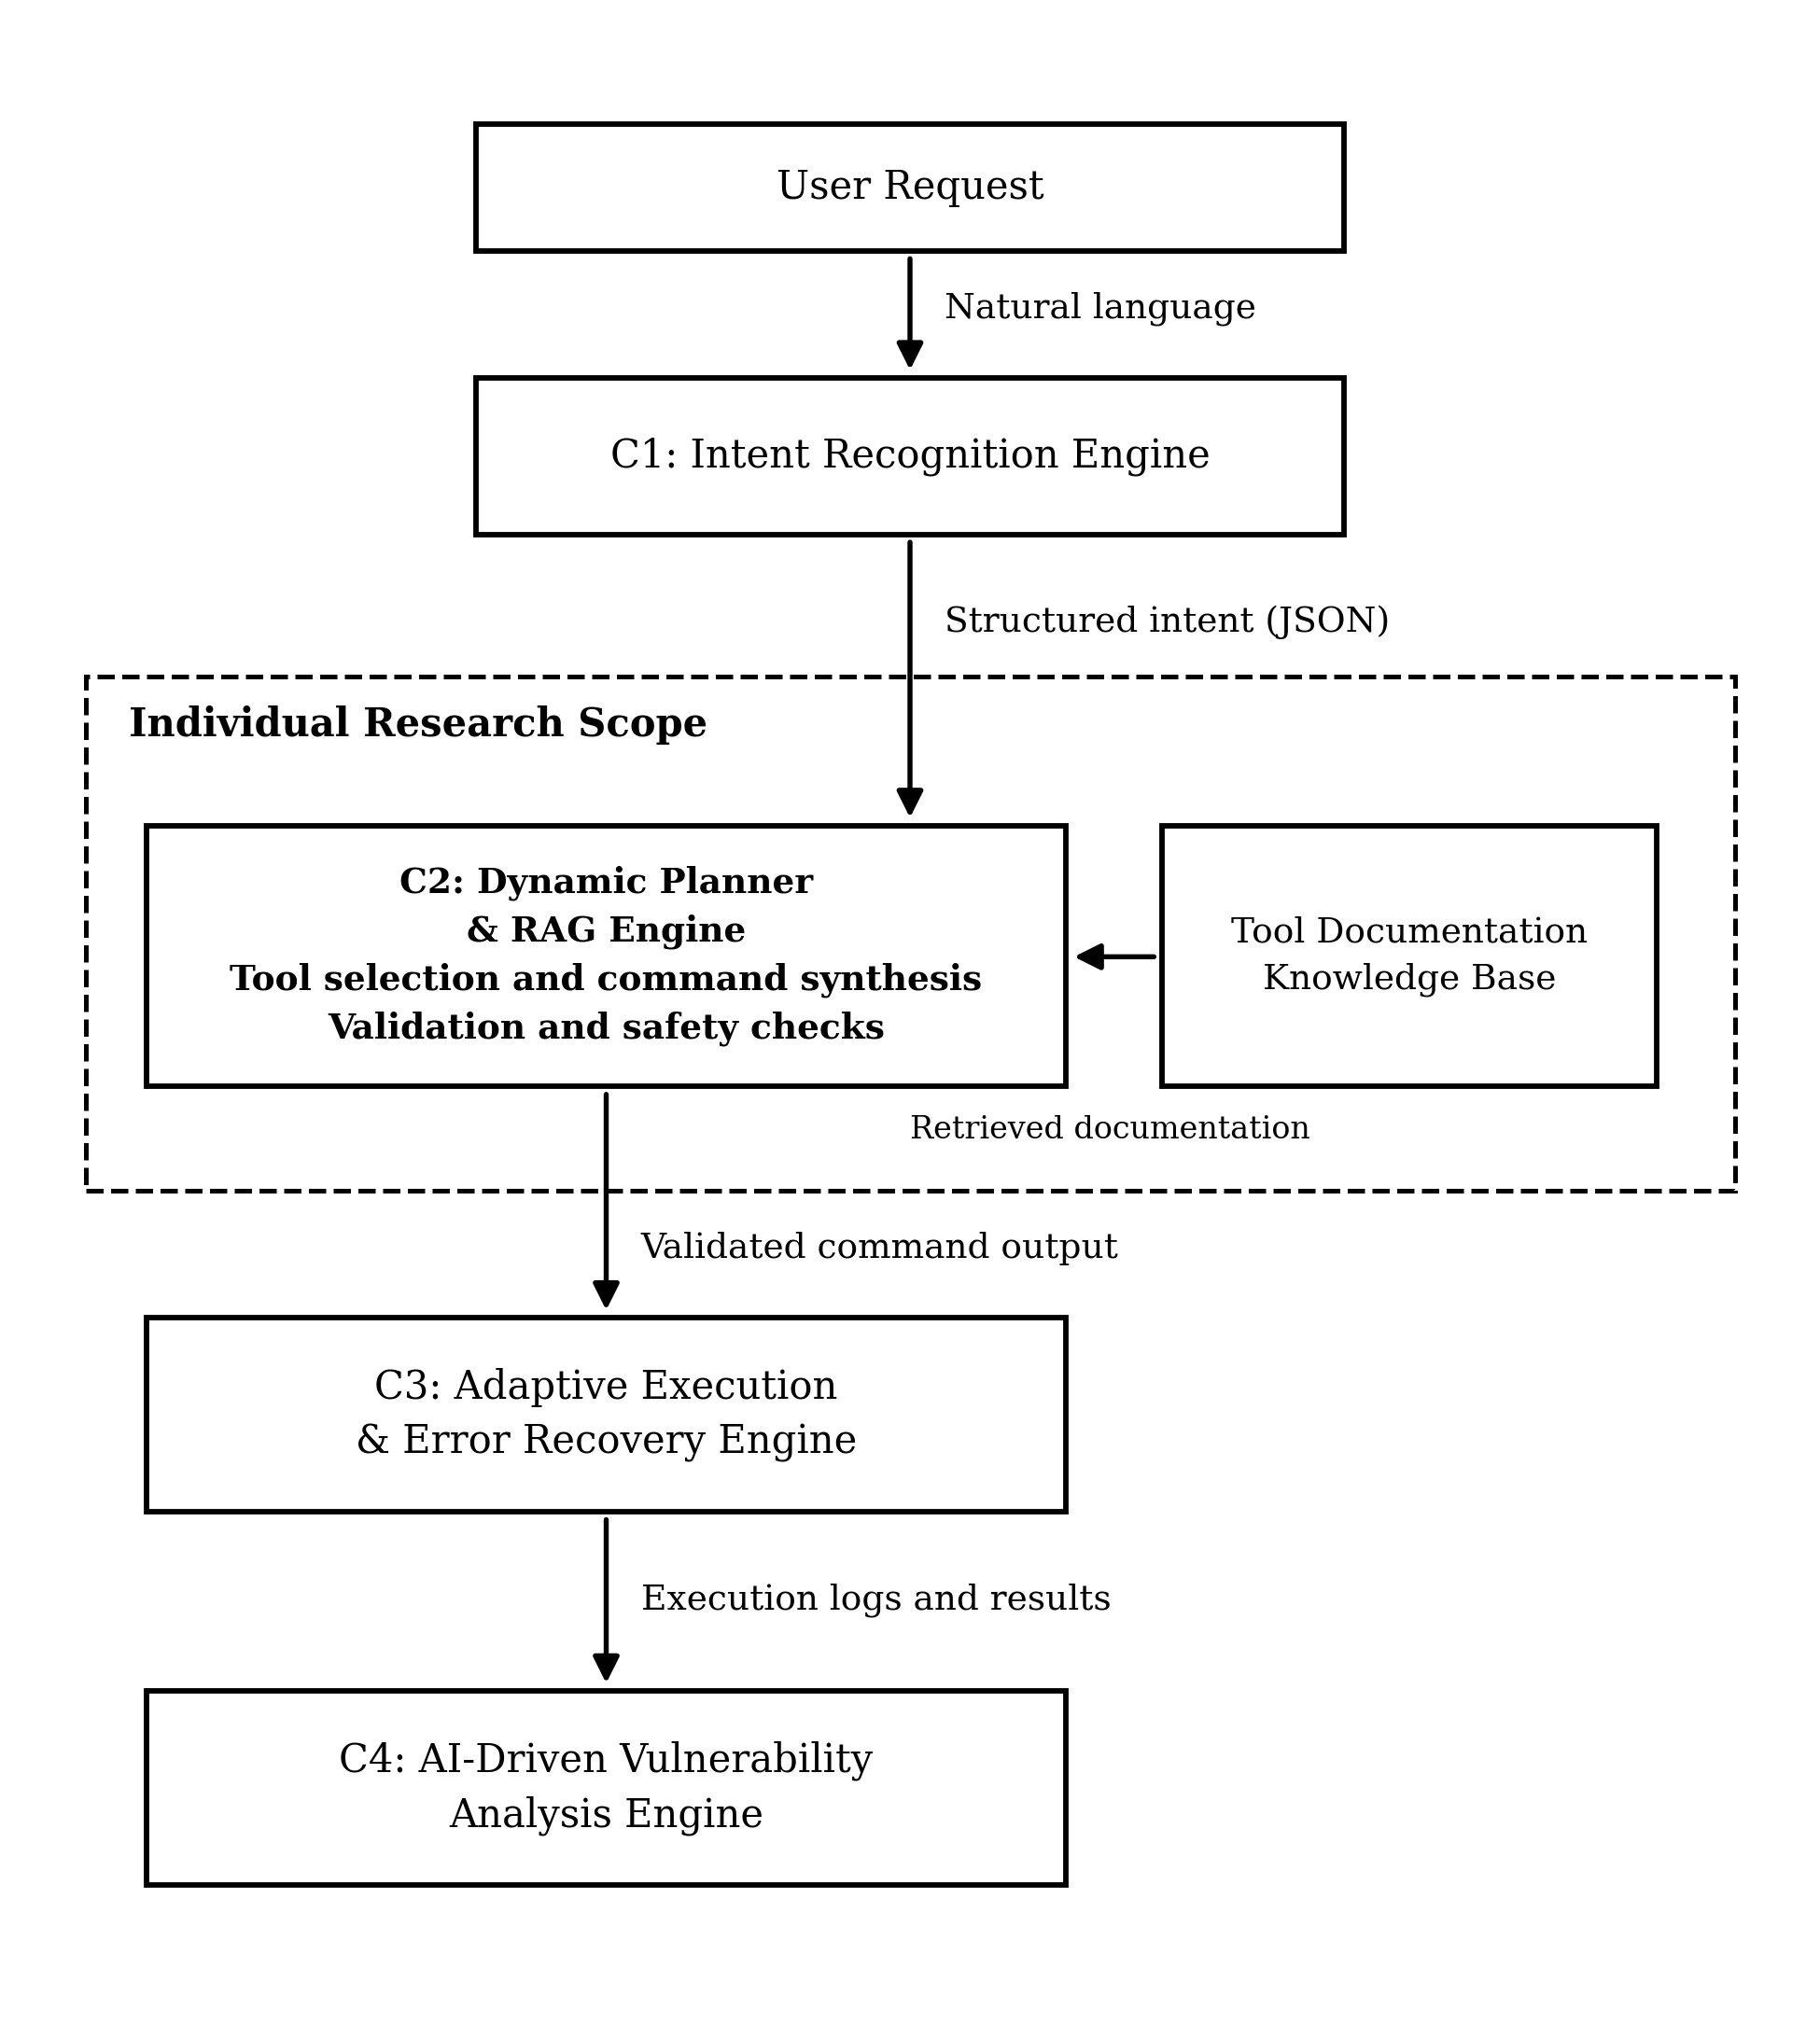
\includegraphics[width=5.70903in,height=6.35in]{vertopal_80eb40840323498cb949d017d9b2b63a/media/image1.png}

\protect\hypertarget{_Toc242369079}{}{}\emph{Figure 1 NeuroShell
component workflow and the scope of Component 2}

\hypertarget{individual-component-context}{%
\subsection{Individual component
context}\label{individual-component-context}}

The Dynamic Planner and Retrieval-Augmented Generation Engine addresses
the transition from a structured cybersecurity task to command-line
instruction. Recognising a task does not, by itself, establish how that
task should be performed. The planner must select a suitable tool,
preserve the supplied target and operational parameters, and express the
requested behaviour using the syntax supported by that tool. This
translation forms the central focus of the individual research
component.

The component combines structured intent processing with retrieval of
relevant tool documentation. The knowledge base contains documentation
and usage information for the supported tools. During planning, relevant
passages are retrieved and supplied as context for command synthesis.
This approach provides the generation stage with an explicit reference
for tool options and usage, while allowing the documentation collection
to be maintained separately from the language model.

\hypertarget{problem-statement}{%
\subsection{Problem statement}\label{problem-statement}}

The problem addressed in this research is how to translate a structured
cybersecurity intent into a command that accurately represents the
requested operation and satisfies the constraints of the supported tool
environment. Identifying the task category is only part of this process.
The planner must also preserve the target, incorporate the requested
parameters, select compatible options, and produce an output that can be
checked before execution

Command correctness has several dimensions. A command may use valid
syntax while performing a different operation from the one requested.
For example, a network-scanning command may identify the correct target
but omit the specified ports or fail to apply a requested scan option.
Conversely, a command may reflect the intended operation but contain an
unsupported argument or an incorrectly formatted parameter. Evaluating
syntax alone would therefore provide an incomplete assessment of the
planner's reliability.

\hypertarget{research-gap}{%
\subsection{Research gap}\label{research-gap}}

Research on large language models in penetration testing has
demonstrated their potential to support tool use, interpret execution
output, and propose subsequent actions. PentestGPT, for example,
investigates these capabilities within a broader penetration-testing
workflow and identifies difficulties in maintaining the context of an
entire testing scenario . This provides an important foundation for
cybersecurity automation. However, the present study addresses a more
specific unit of analysis: the translation of an explicit structured
intent into a validated command.

\hypertarget{aim-and-objectives}{%
\subsection{Aim and objectives}\label{aim-and-objectives}}

The aim of this research is to design, develop, and evaluate a Dynamic
Planner and Retrieval-Augmented Generation Engine that translates
structured cybersecurity intents into commands grounded in tool
documentation and checked against explicit validation and safety
constraints. The study focuses on Nmap, Nikto, and Gobuster within the
NeuroShell framework.

To design a planning workflow that processes the structured intent
contract supplied by the Intent Recognition Engine and identifies the
task, target, and operational parameters required for command
generation.

To develop a retrievable knowledge base containing documentation for
Nmap, Nikto, and Gobuster, and integrate retrieval of relevant passages
into the command-synthesis workflow.

To implement tool selection and command synthesis that combine
structured task information with retrieved documentation while
preserving the requested target, ports, and supported modifiers.

To implement validation and safety checks that examine generated
commands and reject outputs or requests that violate the component's
supported rules and operational constraints.

To integrate the planner with the NeuroShell component interfaces
through an API that accepts structured intent and returns command output
with relevant planning and validation metadata.

To evaluate the component using defined test cases and comparison
configurations, considering tool selection accuracy, command syntax
correctness, semantic alignment, safety behaviour, and generation
latency.

\hypertarget{research-questions-or-hypotheses}{%
\subsection{Research questions or
hypotheses}\label{research-questions-or-hypotheses}}

\begin{enumerate}
\def\labelenumi{\arabic{enumi}.}
\item
  RQ1: How accurately does the planner translate structured
  cybersecurity intents into commands that select the appropriate tool,
  preserve the supplied operational parameters, and represent the
  requested task using valid syntax?
\item
  RQ2: What effect does retrieval of tool documentation have on command
  correctness and generation latency compared with an otherwise
  equivalent configuration that does not use retrieved documentation?
\item
  RQ3: How effectively do the validation and safety mechanisms reject
  invalid commands and requests that violate configured constraints
  while allowing valid, in-scope requests to proceed?
\item
  RQ4: How reliably does the planner maintain its structured input and
  output contract when operating through the API and interacting with
  the surrounding NeuroShell components?
\end{enumerate}

\hypertarget{scope-limitations-and-assumptions}{%
\subsection{Scope limitations and
assumptions}\label{scope-limitations-and-assumptions}}

The component accepts structured intent through its API and processes
the task category, target information, and supported operational
parameters. Its responsibilities include tool selection, retrieval of
relevant documentation, command synthesis, validation, and the
preparation of structured output for the execution component.

The supported tools are Nmap, Nikto, and Gobuster, corresponding to
network scanning, web vulnerability auditing, and directory enumeration.
The study examines command generation within these task categories and
the options supported by the implementation. It does not assume that
every feature of each tool is covered.

Natural language intent recognition is the responsibility of Component
1. The planner consumes the resulting structured contract rather than
performing the complete interpretation of the original user request.
Although the planner checks and processes incoming fields, it cannot
independently establish that those fields accurately capture every
detail of the user's original intention.

The findings are limited to the supported tools, documented options, and
cases included in the evaluation. Performance on these cases does not
establish equivalent performance on unfamiliar tools, unrestricted shell
commands, or complete autonomous penetration-testing scenarios

\hypertarget{individual-contribution}{%
\subsection{\texorpdfstring{ Individual
contribution}{ Individual contribution}}\label{individual-contribution}}

My individual contribution to NeuroShell is the design and development
of Component 2, the Dynamic Planner and Retrieval-Augmented Generation
Engine. This component connects structured intent recognition with
command execution by translating a task contract into command
instructions and examining the generated output against supported
validation and safety constraints.

The contribution includes the organisation of the planning workflow into
distinct stages for intent processing, documentation retrieval, tool
selection, command synthesis, and validation. This separation makes the
responsibilities of each stage explicit and provides a basis for
investigating failures within the planning process. It also allows the
component to be developed and tested through structured inputs without
requiring the complete framework to be active for every test.

\hypertarget{thesis-structure}{%
\subsection{Thesis structure}\label{thesis-structure}}

Chapters 2 and 3 establish the related work and research method.
Chapters 4 and 5 describe the solution design, implementation,
integration, and testing. Chapter 6 reports results, followed by their
interpretation and limitations in Chapter 7. Chapter 8 considers
commercialisation and sustainability. Chapter 9 concludes the study and
identifies future work. References and appendices provide the cited
literature and supporting material.

\hypertarget{literature-review-and-related-work}{%
\section{\texorpdfstring{ LITERATURE REVIEW AND RELATED
WORK}{ LITERATURE REVIEW AND RELATED WORK}}\label{literature-review-and-related-work}}

\hypertarget{review-method-and-scope}{%
\subsection{\texorpdfstring{ Review method and
scope}{ Review method and scope}}\label{review-method-and-scope}}

The review focused on work relevant to translating structured tasks into
tool commands. It considered language-model-assisted penetration
testing, natural-language-to-command translation, retrieval-augmented
generation, sentence embeddings, and command injection prevention. The
sources were selected for their relevance to the component boundary and
design decisions rather than to establish a comprehensive review of
cybersecurity automation.

Primary research publications and technical guidance were examined. The
discussion distinguishes findings established in those sources from
design interpretations made for NeuroShell. The chapter presents a
focused narrative review of the sources relevant to the planning
component.

\hypertarget{domain-and-theoretical-foundations}{%
\subsection{\texorpdfstring{ Domain and theoretical
foundations}{ Domain and theoretical foundations}}\label{domain-and-theoretical-foundations}}

Command planning translates a task representation into the syntax of a
selected utility. The output must retain the destination, requested
operation, ports, and significant modifiers. Syntactic validity alone is
insufficient: a valid command can scan the wrong destination or omit a
required option. Structured input makes these requirements available for
explicit checking, although it remains dependent on the correctness of
upstream intent interpretation.

Retrieval and model adaptation address different parts of this problem.
Retrieval supplies documentation relevant to the current operation;
adaptation teaches the model a specialised input-to-output pattern. LoRA
freezes pretrained weights and introduces trainable low-rank updates
{[}6{]}. In this study, its role was to adapt Gemma to the structured
command-generation task. It did not remove the need to verify the
command or the examples used for adaptation.

\hypertarget{related-research}{%
\subsection{Related research}\label{related-research}}

Deng et al. introduced PentestGPT to support penetration-testing
activities through interacting modules {[}1{]}. Their work identified
difficulty maintaining the broader testing context. It motivates
separating responsibilities within an assisted security workflow.
NeuroShell applies that reasoning to a narrower planning boundary:
Component 2 receives structured intent and returns a checked command.
PentestGPT evaluates testing workflows, whereas this study principally
evaluates command outputs; their reported performance measures are
therefore not directly comparable.

Lin et al. presented NL2Bash, a corpus and semantic parsing approach for
mapping English descriptions to Bash commands {[}2{]}. This establishes
task-to-command translation as a distinct research problem. Component 2
differs because natural-language interpretation occurs upstream. Its
input already contains explicit fields, allowing the generated
executable and arguments to be compared with the requested operation.

Lewis et al. combined parametric generation with retrievable knowledge
for knowledge-intensive NLP tasks {[}3{]}. The relevant principle is
that external evidence can inform generation. NeuroShell uses retrieved
documentation in the prompt rather than reproducing their jointly
trained architecture. Documentation can clarify an option or argument,
but an illustrative host in a retrieved example must not replace the
request target.

Reimers and Gurevych introduced Sentence-BERT for sentence embeddings
that can be compared using cosine similarity {[}4{]}. This supports the
rationale for embedding-based documentation retrieval. It does not
establish retrieval quality for these security tools. A passage may be
semantically related to a task while lacking the argument needed to
construct its command.

\hypertarget{existing-systems-products-and-techniques}{%
\subsection{Existing systems products and
techniques}\label{existing-systems-products-and-techniques}}

Existing techniques provide complementary capabilities. A language model
can propose commands from task information; a documentation retriever
can supply external context; a parser can examine selected arguments;
and policy rules can restrict supported tools or destinations. Their
combination makes a planning decision easier to inspect, but introduces
dependencies on the quality of documentation, the prompt, and the
implemented checks.

OWASP recommends separating commands from arguments and validating both
against permitted values when operating-system command invocation is
necessary {[}5{]}. Escaping shell metacharacters alone does not prevent
argument injection. For NeuroShell, this supports examining tool
identity and arguments separately. The planner generates commands; the
execution component must additionally use an appropriate process
interface, privileges, and approval controls.

\protect\hypertarget{_Toc242369086}{}{}\emph{Table 2.1 Relationship
between reviewed approaches and the planner}

\begin{longtable}[]{@{}
  >{\raggedright\arraybackslash}p{(\columnwidth - 4\tabcolsep) * \real{0.3333}}
  >{\raggedright\arraybackslash}p{(\columnwidth - 4\tabcolsep) * \real{0.3333}}
  >{\raggedright\arraybackslash}p{(\columnwidth - 4\tabcolsep) * \real{0.3333}}@{}}
\toprule()
\begin{minipage}[b]{\linewidth}\raggedright
\textbf{Approach}
\end{minipage} & \begin{minipage}[b]{\linewidth}\raggedright
\textbf{Relevance}
\end{minipage} & \begin{minipage}[b]{\linewidth}\raggedright
\textbf{Boundary}
\end{minipage} \\
\midrule()
\endhead
PentestGPT {[}1{]} & Modular assistance and task context & Whole testing
workflows \\
NL2Bash {[}3{]} & Task-to-command translation & English input rather
than structured intent \\
RAG {[}2{]} & External evidence for generation & Different architecture
and task domain \\
Sentence-BERT {[}4{]} & Embedding-based similarity & Similarity does not
prove syntax coverage \\
OWASP guidance & Command and argument validation & Execution controls
remain necessary \\
\bottomrule()
\end{longtable}

\hypertarget{gap-synthesis-and-conceptual-framework}{%
\subsection{2.5 Gap synthesis and conceptual
framework}\label{gap-synthesis-and-conceptual-framework}}

The reviewed literature provides foundations for language-model-assisted
cybersecurity, task-to-command translation, and retrieval-supported
generation. However, the sources examined in this chapter do not
directly evaluate the combination required by NeuroShell Component 2:
translating structured cybersecurity intents into commands for Nmap,
Nikto, and Gobuster while preserving supplied parameters and applying
explicit validation constraints. This is a gap within the reviewed
evidence, rather than a claim that no other system addresses similar
requirements.

PentestGPT investigates assistance across a penetration-testing
workflow, whereas NL2Bash examines the translation of English
descriptions into Bash commands {[}1{]}, {[}2{]}. Both are relevant to
the planning problem, but neither provides direct evidence for the
structured interface considered here. Component 2 receives an intent
that has already been recognised, together with task parameters. Its
evaluation must therefore distinguish errors introduced during command
planning from errors originating in intent recognition or execution.

The conceptual framework connects four observable stages: a structured
request defines requirements; retrieval supplies tool context; synthesis
proposes a command; and validation checks the proposal against task and
policy constraints. Evaluation examines each stage through complementary
metrics rather than treating tool selection or reference agreement as
proof of complete correctness.

\hypertarget{research-methodology}{%
\section{RESEARCH METHODOLOGY}\label{research-methodology}}

\hypertarget{research-design}{%
\subsection{Research design}\label{research-design}}

This research takes an applied approach to the problem of translating
structured cybersecurity intents into command-line instructions. The
central artefact is the Dynamic Planner and Retrieval-Augmented
Generation Engine, developed as Component 2 of the NeuroShell framework.
The investigation connects the design of this component with an
assessment of its behaviour on defined planning tasks.

The study treats development and evaluation as related but distinct
activities. Development concerns how structured input, retrieved
documentation, command synthesis, and validation are brought together
within the planner. Evaluation concerns whether the resulting output
satisfies the task requirements. A functioning API or a successfully
generated command is therefore not sufficient evidence of command
correctness; the output must be examined against the supplied intent and
parameters.

The research process connects problem definition, data preparation,
component development, testing, and evaluation. These activities serve
different purposes, but decisions made in one stage affect the others.
For example, the supported task categories determine which documentation
is needed, while the input schema determines which parameters must be
preserved in the generated command.

The study follows an artefact-centred Design Science Research approach
{[}7{]}. The implemented planner is the research artefact. Its
evaluation combines controlled model comparisons, a separate retrieval
ablation, and software verification. These evidence streams answer
different questions and are analysed separately.

\hypertarget{data-participants-or-study-materials}{%
\subsection{Data participants or study
materials}\label{data-participants-or-study-materials}}

The research used data for three purposes: supplying technical knowledge
to the retrieval pipeline, providing command examples for development
and model adaptation, and evaluating the planner. These purposes
required different kinds of evidence. An example that illustrates tool
syntax may be useful during development without providing a complete
task description or a reliable reference command for evaluation.

The consolidated candidate pool contained \textbf{9,391 records}
represented as shell commands. Recorded source labels included
\textbf{UCI KYPO, Pentest-R1 Chat, PentestingCommandLogic, a historical
UKA snapshot, Cyber-SFT-Agent-Qwen38 v3.1, and documentation-derived
Nikto examples}. This pool contained material available for further
preparation; it did not represent the number of examples used to train
the final model. Both synthetic and non-synthetic examples were
included.

The prepared records paired a structured planner input with a reference
command. Each input described the intent, sub-intent, target, ports,
modifiers, and requested tool. The reference command provided the
corresponding output for supervised adaptation or evaluation. This
format reflected Component 2's role in converting a structured task into
a security command.

Provenance fields retained source labels, evidence categories, synthetic
indicators, and origin references where available. They supported
tracing examples to their recorded origins, although they did not
establish that every command had been executed or independently
verified. Converting a tool-call example into a shell command also did
not change whether the original material was synthetic or observed.

Following preparation, the final supervised dataset contained 3,379
input--command pairs. Of these, 2,704 were allocated to training, 338 to
validation, and 337 to held-out testing. The partitions supported
adapter optimisation, development assessment, and final direct model
evaluation, respectively.

The training partition included 918 Nmap, 930 Nikto, and 856 Gobuster
examples. These counts provided broadly similar representation across
the supported tools, but did not establish equal coverage of
sub-intents, parameter combinations, or source types. Tool-level
representation was therefore considered separately from the diversity of
tasks within each tool.

Semantic-template overlap checks were considered during preparation.
However, these checks did not independently establish separation between
every related source conversation or task family. Reference quality also
remained relevant: inspected examples included inconsistent targets and
incomplete option values. Evaluation findings were therefore interpreted
with attention to both the generated command and the quality of its
reference.

\hypertarget{experimental-or-study-procedure}{%
\subsection{Experimental or study
procedure}\label{experimental-or-study-procedure}}

Data preparation involved organising command material into a consistent
representation suitable for Component 2. The consolidated records used a
shell-command representation, while the prepared supervised examples
contained separate input, output, and provenance fields. This structure
allowed the task description, expected command, and source information
to be examined independently.

The structured input recorded the intent, sub-intent, target type and
value, ports, modifiers, and tool hint. The output field contained the
expected command. During supervised dataset construction, the input was
serialised as JSON within a consistent instruction prompt, and
surrounding whitespace was removed from the expected command. The
tokenizer's chat template was then used to format the prompt for the
selected model. These steps standardised the training representation
without establishing that every expected command was semantically
correct.

The preparation records also contained semantic templates and signatures
describing command patterns and modifiers. These fields provided
additional information for examining repetition beyond literal command
strings. Commands that differ only in their target can represent the
same underlying operation, while commands with similar wording may
request different options. The notebook included a comparison of
training and validation semantic-template sets; partitioning and overlap
checks are discussed further in Section 3.2.

For the paired direct-model comparison, the same saved test inputs and
prompt construction were used with the adapter enabled and disabled.
JSON fields were serialised with sorted keys, placed in the shared user
instruction, and formatted through the tokenizer chat template.
Generation used greedy decoding with a 96-token limit. Each continuation
was saved with its index, input, reference, and prediction. The test set
was not used as a training partition.

The separate retrieval ablation compared Base Gemma without RAG and Base
Gemma with Chroma retrieval on 25 cases. Its semantic score and planning
times were read from the saved ablation results. It did not assess the
final adapted model on the 337-case test set. Backend verification used
five selected pytest files covering the API, command validator, safety
filter, intent interpreter, and evaluator.

\hypertarget{measures-and-evaluation-metrics}{%
\subsection{Measures and evaluation
metrics}\label{measures-and-evaluation-metrics}}

Tool-selection accuracy is the percentage of assessed predictions whose
executable is the requested tool. A permitted prefix such as sudo does
not change executable identity. Mentioning a tool in an explanation is
insufficient. Empty responses or outputs without an identifiable
supported executable count as unsuccessful selections.

Exact-match rate is the percentage whose generated command equals the
reference after trimming outer whitespace. This strict measure records
textual agreement. It can penalise code fences, equivalent option forms,
or harmless argument ordering, while a defective reference can reward an
invalid command. It is therefore reported separately from semantic
correctness.

Target preservation concerns the actual target operand, including a
relevant URL port or CIDR prefix. Parameter coverage concerns requested
ports and supported modifiers in their proper argument positions. A
number appearing in a wordlist path or thread count must not be
interpreted as a scan port. Semantic evaluation checks these
relationships through the supported command parser.

Rejection outcomes record whether the configured checks accept valid
supported cases and reject invalid or restricted cases. Planning latency
describes elapsed time for the measured planning path, not scan
execution time. The final held-out prediction records did not provide a
verified aggregate latency measurement.

For each proportion, rate = successful assessed cases / total assessed
cases × 100. The denominator and configuration are retained with the
result. A software-test pass rate describes the selected verification
suite rather than a model accuracy or universal safety rate

\hypertarget{data-analysis}{%
\subsection{\texorpdfstring{ Data
analysis}{ Data analysis}}\label{data-analysis}}

The evaluation separates direct model predictions from the responses
produced by the integrated backend. This distinction helps identify
whether an observed outcome originates from model generation or from
later processing, validation, and policy checks.

For direct model evaluation, the base and adapted models receive the
same structured inputs from the frozen held-out test set. The prompt
follows the format used during training, with the planner input
serialised as JSON. Generation uses deterministic decoding with sampling
disabled and a maximum of 96 new tokens. The base-model configuration
disables the trained adapter, while the adapted configuration enables
it.

Each prediction is saved with its record index, structured input,
expected command, and tool identifier. Predictions are written
incrementally so that completed records remain available if the Colab
session disconnects. Before calculating aggregate results, the saved
records must be checked for missing or duplicate indices and alignment
with the test set.

Predictions were paired by saved index and corresponding input. Overall
and per-tool exact-match rates were calculated from the final records,
and strict base-model agreement was reported under the same scoring
rule. Non-matching outputs were examined to distinguish missing
requirements, alternative syntax, formatting differences, and reference
defects. This review was not a complete independent semantic
adjudication of every final prediction.

\hypertarget{ethics-privacy-security-and-responsible-ai}{%
\subsection{\texorpdfstring{ Ethics privacy security and responsible
AI}{ Ethics privacy security and responsible AI}}\label{ethics-privacy-security-and-responsible-ai}}

NeuroShell Component 2 is designed to support authorised cybersecurity
tasks. Its role is to translate structured intent into a security
command and assess that command before returning it to the wider
framework. Command execution belongs to a separate component and
requires its own operational controls.

The model-generation and API checks described in this study assess
command text and planning behaviour. Generating a command containing a
target address does not involve contacting that target. These checks are
therefore distinguished from scans or enumeration activities performed
against an actual system. Any execution-based testing must remain within
an explicitly authorised environment and agreed scope.

The backend applies target restrictions and command-validation checks to
reduce the chance of returning an unsuitable command. These controls
support responsible use, but they do not establish permission to test a
system. A private IP address alone is not evidence of authorisation; the
operator remains responsible for confirming ownership or permission
before execution.

Tests were framed around authorised laboratory activity. A
private-address restriction is a technical scope rule and does not
establish ownership or consent. Requests, commands, and session records
can reveal internal system details, so access and retention arrangements
are necessary in any deployment. Generative AI assistance in preparing
the dissertation is disclosed in Appendix B.

\hypertarget{reproducibility-and-research-artefacts}{%
\subsection{Reproducibility and research
artefacts}\label{reproducibility-and-research-artefacts}}

The reproducibility record includes structured dataset partitions,
prediction JSONL files, provenance fields, saved adapter and tokenizer
files, merged model artefacts, the local model configuration, backend
source, and selected test output. The two final prediction files are
\emph{\textbf{c2\_final\_test\_predictions.jsonl}} and
\emph{\textbf{c2\_base\_model\_test\_predictions.jsonl}}. Their recorded
location is \emph{\textbf{/content/drive/MyDrive/NeuroShell\_C2/.}}

A reproduction should preserve the model and adapter versions, prompt
text, tokenizer template, decoding settings, test file, scoring rule,
and software environment. Local deployment also depends on \emph{the
GGUF conversion}, \emph{Ollama template}, \emph{knowledge-base
contents}, and \emph{validation configuration}. Changing these creates a
revised configuration whose results must be evaluated separately.
Appendix A provides a compact input example and the verification
command.

\hypertarget{product-and-solution-design}{%
\section{PRODUCT AND SOLUTION
DESIGN}\label{product-and-solution-design}}

\hypertarget{requirements}{%
\subsection{Requirements}\label{requirements}}

The requirements of Component 2 follow its role as the planning stage of
NeuroShell. It must receive structured intent, identify a supported
tool, and produce a command that preserves the requested target and
operational parameters. It must also provide a clear response when a
request cannot be planned or when a generated command fails validation.

Component 2 supports command planning for Nmap, Nikto, and Gobuster. The
workflow combines the current request with relevant documentation and,
where appropriate, context from the same session. Each stage must
preserve the meaning of the request so that information is not lost
between intent processing and command generation.

The planner must be practical to integrate, maintain, and assess.
Producing a command is only one part of this responsibility: the
component also needs consistent interfaces, controlled access, useful
diagnostic information, and clear behaviour when a dependency fails.

\protect\hypertarget{_Toc242369087}{}{}\emph{Table 4.1 Principal
component requirements}

\begin{longtable}[]{@{}
  >{\raggedright\arraybackslash}p{(\columnwidth - 2\tabcolsep) * \real{0.4999}}
  >{\raggedright\arraybackslash}p{(\columnwidth - 2\tabcolsep) * \real{0.5001}}@{}}
\toprule()
\begin{minipage}[b]{\linewidth}\raggedright
\textbf{Area}
\end{minipage} & \begin{minipage}[b]{\linewidth}\raggedright
\textbf{Requirement}
\end{minipage} \\
\midrule()
\endhead
Input & Accept the structured intent contract and retain explicit
requirements \\
Planning & Select Nmap, Nikto, or Gobuster and generate one command \\
Retrieval & Retrieve documentation associated with the selected tool \\
Validation & Check supported syntax, target, ports, and significant
options \\
Policy & Reject requests outside configured rules \\
Integration & Return success or rejection with inspectable metadata \\
Context & Recover a previous target only where the request permits it \\
\bottomrule()
\end{longtable}

\hypertarget{component-architecture-within-the-complete-solution}{%
\subsection{\texorpdfstring{ Component architecture within the complete
solution}{ Component architecture within the complete solution}}\label{component-architecture-within-the-complete-solution}}

Component 2 occupies the planning stage between intent recognition and
command execution. Component 1 describes the requested task through a
structured intent contract. Component 2 uses that information to
construct and validate a command, which is then made available to
Component 3 for execution and error recovery. Component 4 analyses the
resulting security findings.

Component 2 is organised around a planning workflow coordinated by the
API layer. Separate modules handle intent interpretation, tool
selection, retrieval, context assembly, command synthesis, validation,
and session management. This structure allows each responsibility to be
tested and updated without placing the entire workflow in a single
module.

The API receives the structured request and coordinates the planning
stages. Intent processing extracts the task requirements, while session
context supports target recovery when the current request omits a
destination. Tool selection identifies the supported tool before
retrieval searches its documentation

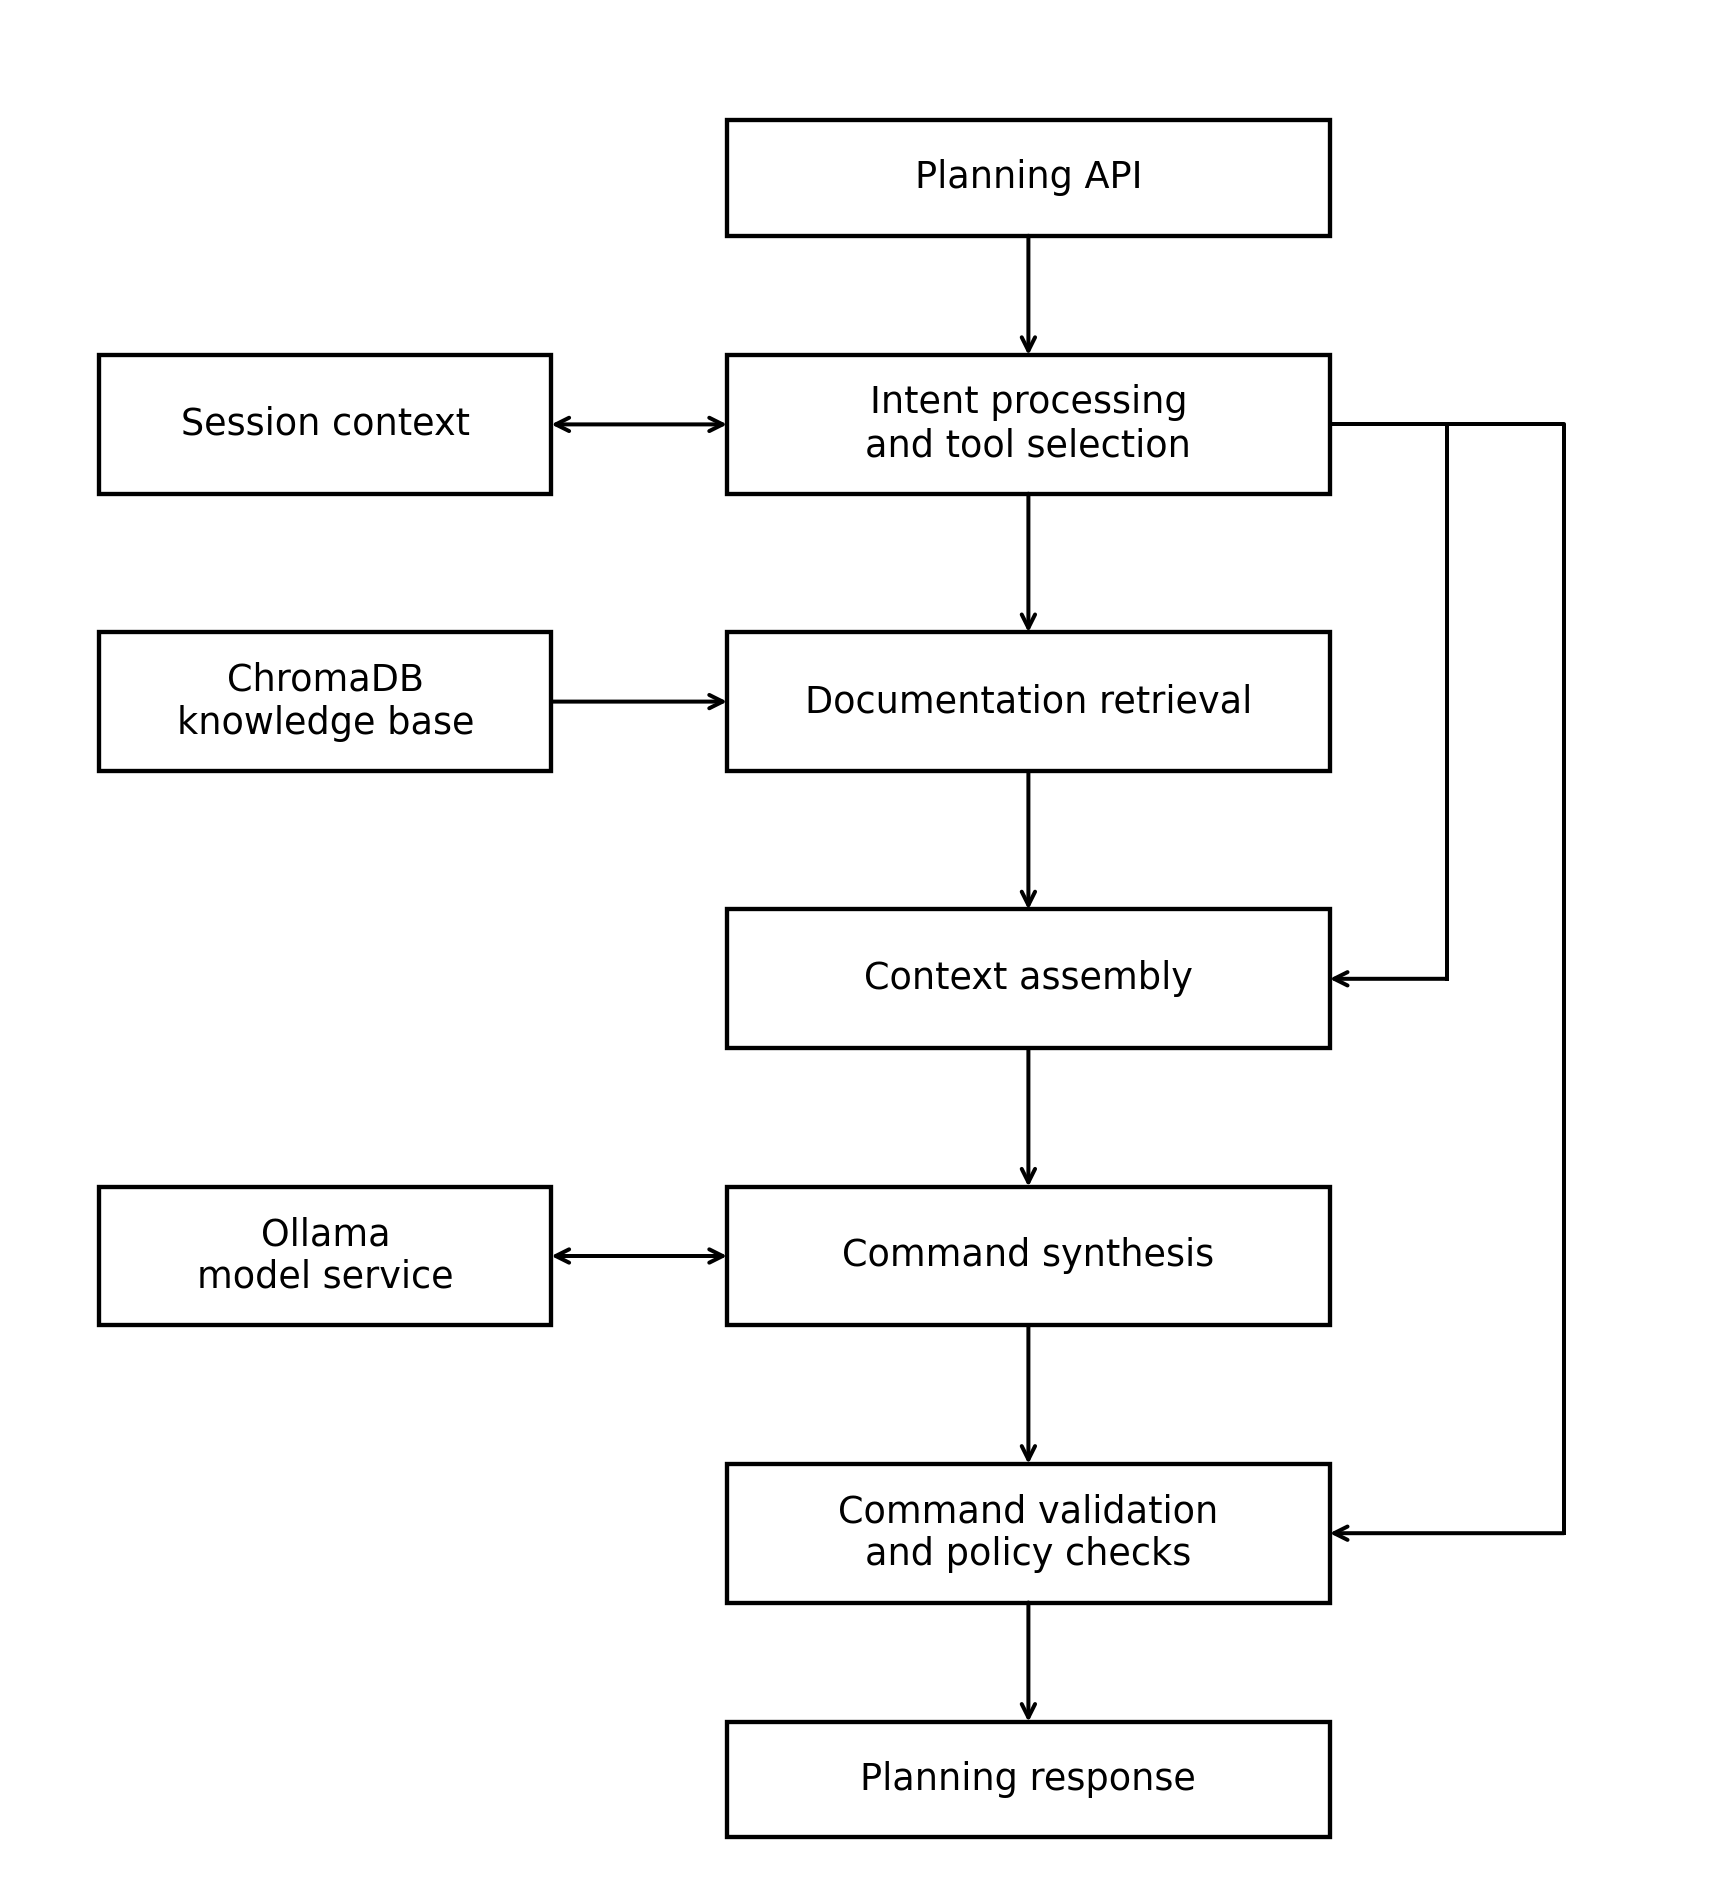
\includegraphics[width=4.99808in,height=5.50634in]{vertopal_80eb40840323498cb949d017d9b2b63a/media/image2.png}

\protect\hypertarget{_Toc242369080}{}{}\emph{Figure 2 Internal
architecture of the Dynamic Planner and RAG Engine}

\hypertarget{design-alternatives-and-decisions}{%
\subsection{Design alternatives and
decisions}\label{design-alternatives-and-decisions}}

The design balances command-generation flexibility with explicit task
requirements and validation. Several choices reflect the project's
supported scope, local deployment needs, and the need to assess failures
clearly.

Using structured intent gives the planner identifiable targets, ports,
and modifiers. These fields can guide generation and serve as validation
inputs. The trade-off is that planning depends on the quality of the
supplied contract: an incomplete or incorrectly interpreted request can
affect the command even when later stages behave as designed.

Model adaptation and documentation retrieval address different needs.
Adaptation teaches the expected relationship between structured requests
and command responses, while retrieval supplies tool information during
planning. Keeping the documentation store separate allows its content to
be updated without retraining. However, retrieval adds processing and
can introduce irrelevant passages, so its contribution must be
evaluated.

A direct generator provides a simple baseline, while retrieval
introduces external documentation and an additional processing path. The
selected design keeps retrieval, synthesis, and validation modular so
that a failure can be examined at its originating stage. Local inference
allows the model to run within the deployment environment, but does not
by itself establish sufficient capacity or confidentiality controls.

\hypertarget{detailed-design}{%
\subsection{Detailed design}\label{detailed-design}}

The input follows the intent contract supplied by Component 1. Its main
fields identify the task, destination, requested parameters, and
preferred tool. Session and confidence information provide additional
context without replacing the task requirements.

The planning workflow turns a structured request into either a validated
command or a clear unsuccessful outcome. Each stage uses the task
information established earlier in the process, allowing the final
command to be checked against the request that produced it.

The workflow begins with authentication and input validation at the API
boundary. The intent interpreter then extracts the target, ports,
modifiers, and task category. If the target is missing, session handling
attempts to recover a suitable destination from the same session. An
explicit target in the current request takes precedence over stored
context.

Intent processing converts the incoming contract into the task
information used throughout planning. It extracts the intent,
sub-intent, target, ports, modifiers, and tool hint while preserving the
caller's requirements. This gives retrieval, generation, and validation
a consistent description of the same task.

Retrieval supplies tool information relevant to the current task before
command generation. The planner searches its documentation knowledge
base using the interpreted intent and selected tool. This gives the
model access to passages about command syntax and options that may help
it construct the requested command

The knowledge base stores documentation passages in ChromaDB with
embeddings produced by the all-MiniLM-L6-v2 model. Each passage includes
source metadata identifying its tool. The retrieval query uses the same
embedding model, and tool filtering narrows the search to documentation
associated with the selected tool.

Command synthesis converts the assembled task context into a candidate
shell command. The synthesizer receives the interpreted request and
relevant documentation, then submits them to the configured model
through Ollama. In the final deployment, the model is identified as
neuroshell-c2-gemma2-final.

The input includes intent, sub\_intent, target type and value, ports,
modifiers, and an optional tool hint. An explicit current target takes
priority over stored session context. Target inference distinguishes
URLs, IP addresses, and subnets where needed. Unsupported or
contradictory requirements should be rejected rather than silently
rewritten. The selected mapping is \textbf{NETWORK\_SCAN} to Nmap,
\textbf{VULNERABILITY\_AUDIT} to Nikto, and
\textbf{DIRECTORY\_BRUTEFORCE} to Gobuster.

Documentation is divided into passages, embedded, and stored in Chroma
with tool metadata. Retrieval is filtered by the selected tool before
the context is assembled. The structured requirements remain
authoritative when a retrieved passage contains example destinations.
The generator returns a proposal, and the validation layers decide
whether it satisfies the implemented checks.

\protect\hypertarget{_Toc242369088}{}{}\emph{Table 4.2 Planning contract
and interfaces}

\begin{longtable}[]{@{}
  >{\raggedright\arraybackslash}p{(\columnwidth - 2\tabcolsep) * \real{0.4999}}
  >{\raggedright\arraybackslash}p{(\columnwidth - 2\tabcolsep) * \real{0.5001}}@{}}
\toprule()
\begin{minipage}[b]{\linewidth}\raggedright
\textbf{Element}
\end{minipage} & \begin{minipage}[b]{\linewidth}\raggedright
\textbf{Role}
\end{minipage} \\
\midrule()
\endhead
POST /plan & Receive a structured planning request \\
x-api-key & Authenticate the caller at the API boundary \\
POST /kb/update & Provide the knowledge-base update interface \\
Planning response & Return command, outcome, and available validation
metadata \\
Rejected response & Explain the supported input or validation failure \\
Session identifier & Associate requests with relevant stored context \\
\bottomrule()
\end{longtable}

\hypertarget{standards-and-professional-practice}{%
\subsection{\texorpdfstring{ Standards and professional
practice}{ Standards and professional practice}}\label{standards-and-professional-practice}}

The design uses explicit contracts, separated responsibilities, and
testable validation rules to make planning decisions inspectable.
Command and argument checking follows the rationale of OWASP guidance
{[}5{]}; this alignment does not constitute a security certification.
Execution must remain subject to destination approval and suitable
process-level controls.

Professional practice also requires clear configuration management.
Model artefacts, prompts, documentation, and validators should be
versioned together because changing one can alter system behaviour.
Documentation provenance should record the source and tool version where
available. In the prototype, tool metadata provides useful filtering,
but richer document-level attribution remains a maintenance improvement.

\hypertarget{implementation-integration-and-testing}{%
\section{\texorpdfstring{ IMPLEMENTATION INTEGRATION AND
TESTING}{ IMPLEMENTATION INTEGRATION AND TESTING}}\label{implementation-integration-and-testing}}

\hypertarget{development-environment-and-technology-stack}{%
\subsection{Development environment and technology
stack}\label{development-environment-and-technology-stack}}

Development used two environments: Google Colab for model adaptation and
direct inference, and a local Windows environment for backend
development and Ollama deployment. This arrangement allowed GPU-based
model work to be carried out separately from the planning service.

The \emph{Colab environment used a Tesla T4 GPU}. The model workflow
combined PyTorch and Transformers for loading and inference, PEFT for
adapter handling, and TRL for supervised fine-tuning. BitsAndBytes
supported quantised model loading during adaptation. The trained adapter
was subsequently merged with the base model, and the merged model was
converted to a \emph{Q8\_0 GGUF} file for local use.

\protect\hypertarget{_Toc242369089}{}{}\emph{Table 5.1 Main
implementation technologies}

\begin{longtable}[]{@{}
  >{\raggedright\arraybackslash}p{(\columnwidth - 2\tabcolsep) * \real{0.4999}}
  >{\raggedright\arraybackslash}p{(\columnwidth - 2\tabcolsep) * \real{0.5001}}@{}}
\toprule()
\begin{minipage}[b]{\linewidth}\raggedright
\textbf{Technology}
\end{minipage} & \begin{minipage}[b]{\linewidth}\raggedright
\textbf{Role}
\end{minipage} \\
\midrule()
\endhead
Python and FastAPI & Planning modules and API \\
Gemma 2 2B instruction model & Base generator \\
LoRA and PEFT & Saved adaptation weights \\
Ollama and Q8\_0 GGUF & Local model inference \\
Sentence Transformers and Chroma & Documentation embeddings and
retrieval \\
Redis with local fallback & Session context \\
pytest & Selected unit and API verification \\
\bottomrule()
\end{longtable}

\hypertarget{component-implementation}{%
\subsection{\texorpdfstring{ Component
implementation}{ Component implementation}}\label{component-implementation}}

The backend code is organised by responsibility under the src directory.
API handling, intent interpretation, retrieval, command synthesis,
validation, and session storage have separate modules. Shared schemas
define the information exchanged between these stages.

Intent processing is implemented in intent\_interpreter.py. The
interpreter receives the structured intent contract and extracts the
task category, target information, ports, modifiers, and tool hint into
an internal representation. This information is then passed to the later
planning stages.

Target-type inference handles requests whose target type is missing or
marked as unknown. URL prefixes identify web destinations, while
Python's ipaddress module distinguishes IP addresses and network-related
values. Other non-empty destination values are treated as domain
candidates. This classification supports subsequent processing but does
not replace target validation or policy checks.

The retrieval pipeline uses documentation for Nmap, Nikto, and Gobuster
stored under knowledge\_base/raw\_docs. These files provide the material
from which searchable passages are constructed. The persistent ChromaDB
store is maintained separately under knowledge\_base/chroma\_db.

During ingestion, documentation is divided into passages with overlap
between adjacent sections. The documented ingestion configuration uses a
character-based chunk size of 512 and an overlap setting of 64. These
values describe text segmentation rather than token counts. Overlap
retains some neighbouring context where an option description or example
crosses a passage boundary.

The final model integration connects the command synthesizer to the
adapted Gemma model served through Ollama. Model preparation took place
in Colab, while the backend uses the exported model locally. This
separates training dependencies from the application's inference
workflow.

The saved adapter was loaded with google/gemma-2-2b-it and merged into
the base model in FP16. The merged weights and tokenizer were saved
together, then converted into a Q8\_0 GGUF file. The file was imported
into Ollama as neuroshell-c2-gemma2-final, using the detected Gemma
instruction template.

The retriever uses all-MiniLM-L6-v2 embeddings. Prepared text passages
use a 512-character chunk size with 64-character overlap. These are
character counts, not token counts. Tool metadata constrains retrieval
to the selected utility. A score derived from cosine distance provides a
ranking signal and must not be interpreted as a calibrated probability
that a command is correct.

The command synthesizer builds the generation context from the
structured request and available documentation. Basic validation checks
output structure and supported tool use. The semantic evaluator parses
supported command forms to compare target operands, ports, and
significant options against the request. The safety filter applies the
configured destination and dangerous-pattern rules. These layers have
distinct responsibilities and are not substitutes for authorised
execution.

Session storage uses Redis when available and an in-memory fallback when
it is unavailable. The fallback belongs to the current API process, so
it cannot be assumed to share state across instances or retain it after
restart. Explicit request targets override recovered context. This
prevents an earlier target from silently replacing a newly supplied
destination.

\hypertarget{integration-with-the-other-components}{%
\subsection{\texorpdfstring{ Integration with the other
components}{ Integration with the other components}}\label{integration-with-the-other-components}}

Component 2 connects intent interpretation with command execution within
the NeuroShell workflow. It receives a structured task from Component 1
and produces a planning response for Component 3. Its responsibility is
to translate the requested task into a command and apply the relevant
validation controls before returning it.

Component 1 supplies the structured intent used by the planner. The
relevant information includes the task category, target, requested
ports, modifiers, and tool hint. Component 2 processes these fields
through its input schema and intent interpreter before retrieval and
command generation.

Preserving these requirements is essential. For example, a request to
scan ports 22, 80, and 443 must retain all three ports throughout the
planning process. The generated command must also express them using the
appropriate tool syntax. An explicit target in the current request takes
precedence over a target retained in session context.

Component 1 supplies the interpreted task. Component 2 returns a command
proposal and planning outcome for Component 3 to handle execution and
recovery. Component 4 handles later analysis. The assessed API contract
connects these responsibilities, but the recorded component tests do not
establish a complete live four-component workflow under all deployment
conditions.

\hypertarget{verification-and-software-testing}{%
\subsection{\texorpdfstring{ Verification and software
testing}{ Verification and software testing}}\label{verification-and-software-testing}}

Testing covered the behaviour of individual modules and the planning
workflow exposed through the API. The approach combined automated checks
with live requests to the locally deployed model. These served different
purposes: automated tests checked specific behaviours under controlled
conditions, while live checks examined the response produced by the
running backend and its dependencies.

Unit tests focused on behaviours that could be checked independently of
the complete API workflow. These included intent interpretation, tool
selection, command validation, and session-context handling. Each case
supplied a defined input and checked the resulting value or decision.

For intent processing, relevant cases covered target-type inference and
preservation of the supplied task requirements. Tool-selection checks
examined the mappings between supported intents and Nmap, Nikto, or
Gobuster, together with the handling of unsupported requests.

API tests examined the planning workflow through the /plan endpoint.
They checked how the application handled authentication, structured
requests, planning decisions, and response construction. This extended
testing beyond individual modules by exercising their interaction within
the backend.

Validation and policy tests examined whether the planner distinguished
acceptable commands from outputs that violated the request or the
configured restrictions. The cases covered command structure, tool
identity, target preservation, requested ports, and destination policy.

Session-related tests examined how the planner handled requests that
depended on previously established context. The main concern was target
recovery: a follow-up request without an explicit destination should use
the appropriate stored target only when suitable context exists for that
session.

The selected run covered 42 tests in five files. Cases examined
authentication failure, rejected intents, public-address blocking,
strict-validator failure, target recovery, malformed quotation marks,
extra targets, URL-port contradictions, CIDR mismatch, and malformed
attached Nmap port arguments. Evaluator tests also addressed false
matches involving a target inside a wordlist path, a thread count
mistaken for a port, and a filename following -iL mistaken for a scan
target.

These checks exercise the supported behaviours under their test
arrangements. Some cases use mocks, so the suite is not a measurement of
live model generation or live command execution. The results are
reported in Section 6.2. The full verification command is retained in
Appendix A.

\hypertarget{deployment-and-operation}{%
\subsection{Deployment and operation}\label{deployment-and-operation}}

Deployment of Component 2 requires resources for model inference, the
planning API, retrieval, and session management. These services need to
operate together so that a structured request can be processed, checked,
and returned to the calling application.

The research used a quantised Q8\_0 model through Ollama for local
inference. The model file occupied approximately 2.8 GB of storage, but
this is not a minimum memory requirement. Runtime memory also depends on
the inference configuration, context length, and workload. Suitable
hardware would therefore need to be selected through measurements using
the intended deployment settings.

The backend also requires its Python environment, application
dependencies, embedding model, and ChromaDB knowledge base. Redis
supports session storage, while the implemented in-memory fallback
provides an alternative when Redis is unavailable. Because process-local
storage is not shared across backend instances, a deployment serving
multiple instances would need a consistent approach to session state.

The saved adapter was loaded with the matching base model, merged into
FP16 weights on CPU, and saved with the tokenizer. The merged model was
converted to the final Q8\_0 GGUF artefact and imported into Ollama as
\emph{\textbf{neuroshell-c2-gemma2-final}}. The GGUF file occupied
approximately 2.8 GB; this is a storage figure, not a minimum runtime
memory specification.

Early local and Colab outputs differed for a ports-only request, and
both omitted the required -p form. A later input containing the explicit
port modifier and a more specific sub-intent produced the correct
command in both environments. Because more than one input field changed,
the observation does not isolate one causal fix or establish overall
export parity. The deployment should preserve the training prompt
structure and be evaluated independently after conversion.

\hypertarget{results-and-validation}{%
\section{\texorpdfstring{ RESULTS AND
VALIDATION}{ RESULTS AND VALIDATION}}\label{results-and-validation}}

\hypertarget{research-results}{%
\subsection{Research results}\label{research-results}}

Direct assessment compared the base and adapted configurations on 337
held-out cases, comprising 113 Nmap, 116 Nikto, and 108 Gobuster cases.
The adapted model achieved an overall strict exact-match rate of
87.54\%. Table 6.1 presents the results by tool.

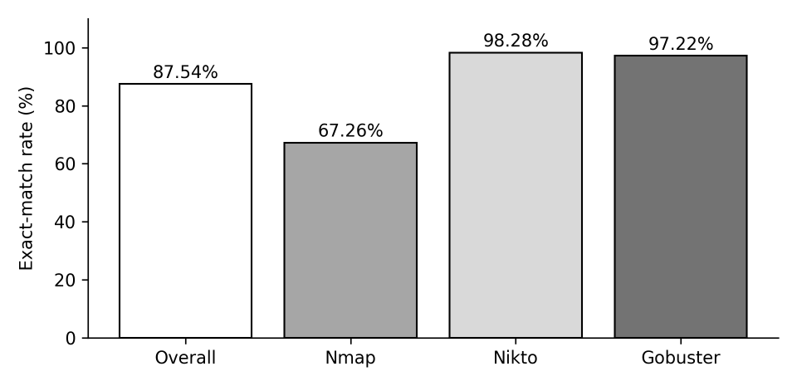
\includegraphics[width=5.31389in,height=2.57361in]{vertopal_80eb40840323498cb949d017d9b2b63a/media/image3.png}

\protect\hypertarget{_Toc242369081}{}{}\emph{Figure 3 Overall and
per-tool exact-match rates on the held-out assessment}

Figure 3 shows that strict exact-match performance varied across the
three tools. Nikto and Gobuster achieved higher rates than Nmap, making
Nmap the main priority for further error analysis. These results apply
to the assessed cases and do not establish equivalent performance across
all tool modes or option combinations. Inspection identified non-matches
involving alternative option forms and incomplete quotation marks in
stored references. The reported rates retain the original reference
commands without adjusting the scores for these differences.

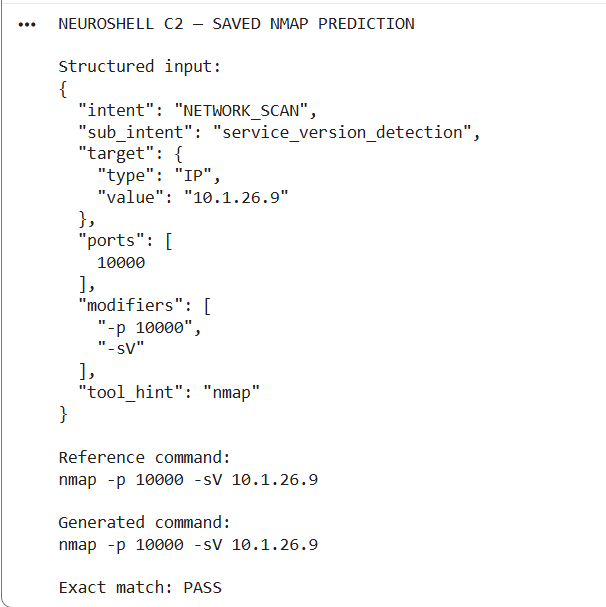
\includegraphics[width=4.35262in,height=4.38981in]{vertopal_80eb40840323498cb949d017d9b2b63a/media/image4.png}

\protect\hypertarget{_Toc242369082}{}{}\emph{Figure 4 Saved Nmap
prediction matching the reference command}

A separate 25-case experiment examined the base model with and without
retrieval. Semantic command accuracy increased from 56\% without
retrieval to 84\% with retrieval, an improvement of 28 percentage
points. Normalised exact-match rates were 12\% and 16\%, respectively,
while tool-selection accuracy remained at 80\% in both configurations.
These findings suggest that documentation grounding improved command
generation under the conditions of that experiment. However, this
comparison was separate from the held-out assessment shown in Figure 3
and did not measure the effect of retrieval on the final adapted model.

\hypertarget{product-and-technical-results}{%
\subsection{Product and technical
results}\label{product-and-technical-results}}

The selected backend verification run passed all 42 tests, with one
warning, in 71.28 seconds. The environment reported Windows, Python
3.11.9, and pytest 8.2.0. The warning concerned a pending deprecation in
the multipart import used through Starlette. It was not a test failure.
The 71.28-second duration describes the suite run, not average API
response time.

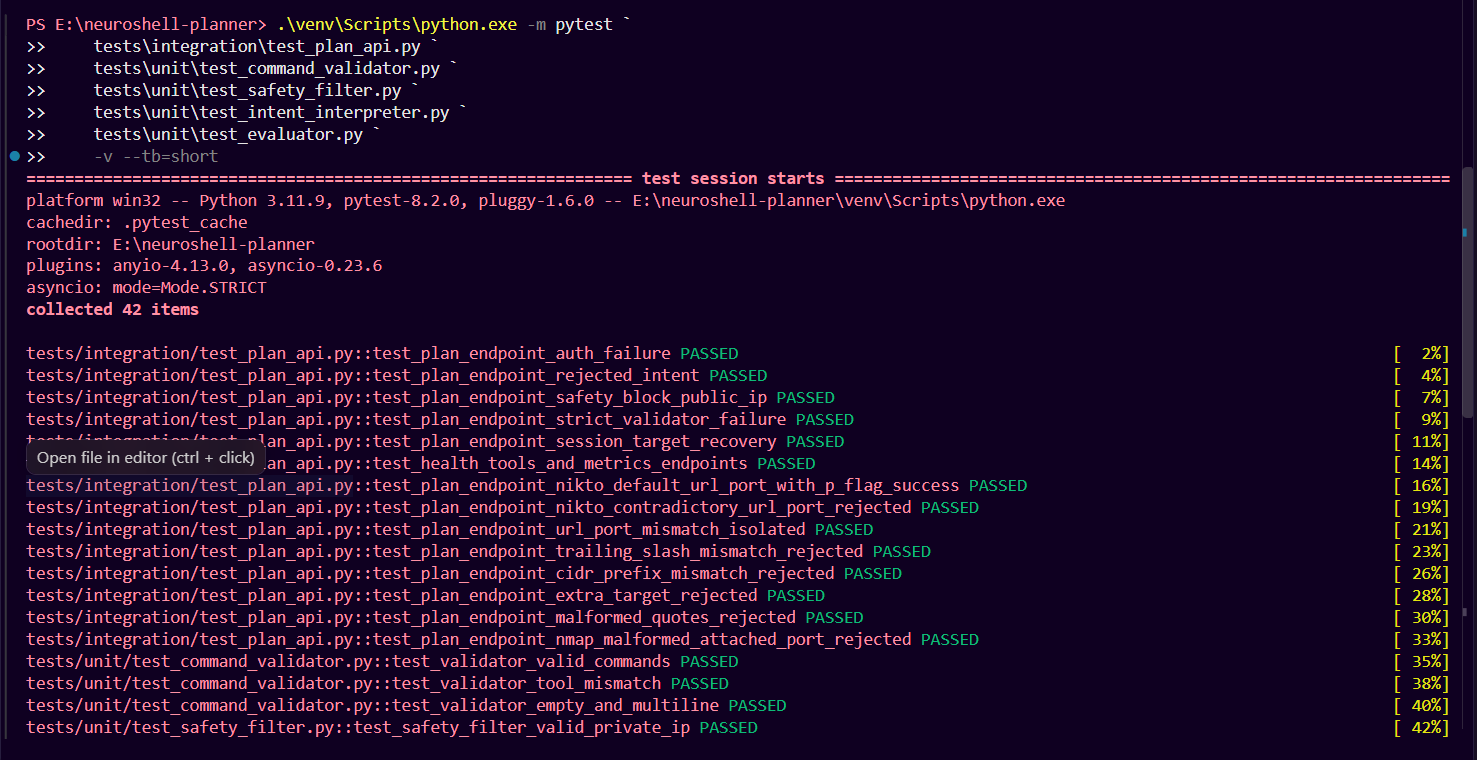
\includegraphics[width=5.70903in,height=2.9375in]{vertopal_80eb40840323498cb949d017d9b2b63a/media/image5.png}

\protect\hypertarget{_Toc242369083}{}{}\emph{Figure 5 Selected unit and
integration test results}

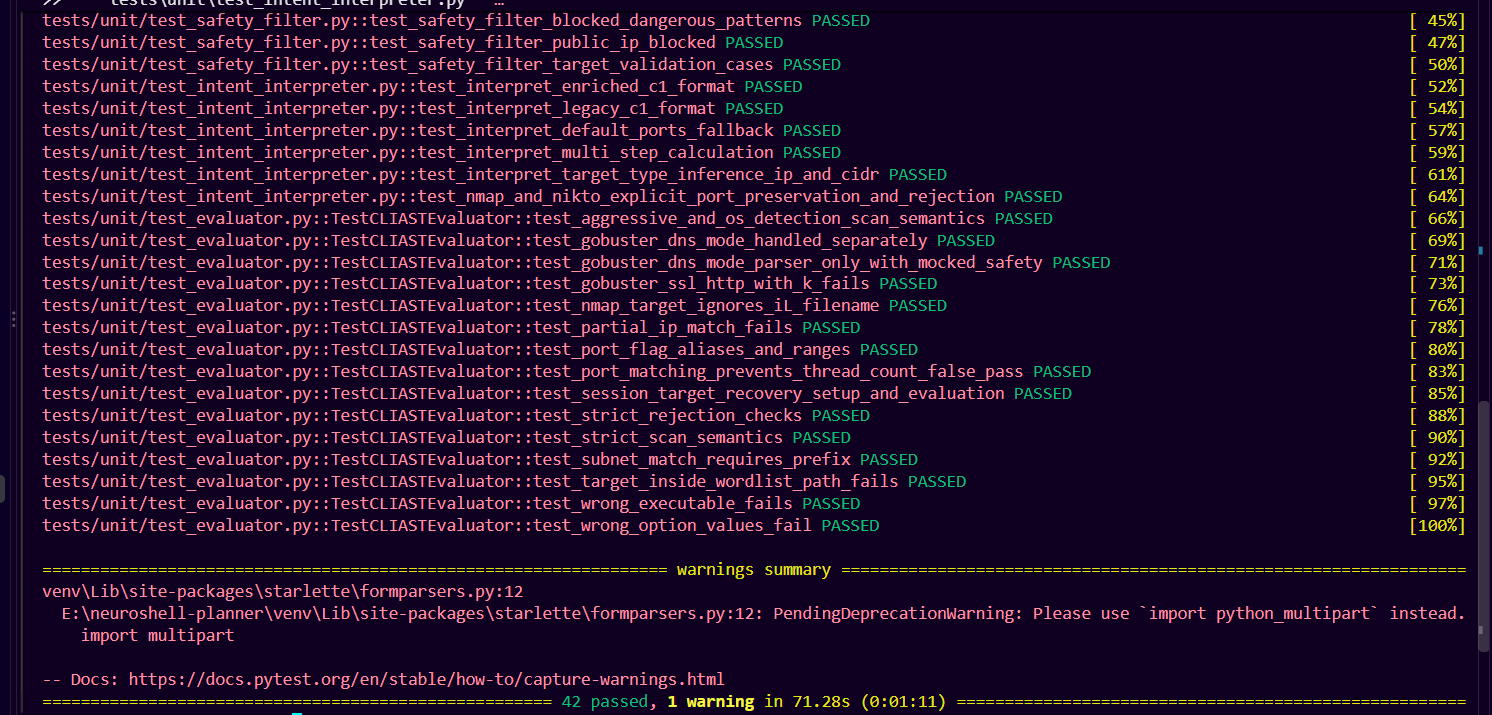
\includegraphics[width=5.70903in,height=2.73542in]{vertopal_80eb40840323498cb949d017d9b2b63a/media/image6.png}

\protect\hypertarget{_Toc242369084}{}{}\emph{Figure 6 est configuration
and initial verification results}

\protect\hypertarget{_Toc242369090}{}{}\emph{Table 6.1 Selected software
verification results}

\begin{longtable}[]{@{}
  >{\raggedright\arraybackslash}p{(\columnwidth - 2\tabcolsep) * \real{0.5001}}
  >{\raggedright\arraybackslash}p{(\columnwidth - 2\tabcolsep) * \real{0.4999}}@{}}
\toprule()
\begin{minipage}[b]{\linewidth}\raggedright
\textbf{Test area}
\end{minipage} & \begin{minipage}[b]{\linewidth}\raggedright
\textbf{Passed tests}
\end{minipage} \\
\midrule()
\endhead
Planning API integration & 14 \\
Command validator & 3 \\
Safety filter & 4 \\
Intent interpreter & 6 \\
Command evaluator & 15 \\
Total & 42 \\
\bottomrule()
\end{longtable}

The passing cases support the implemented checks for the tested
malformed commands, target and port contradictions, authentication
behaviour, and session recovery. They do not establish a universal
rejection rate or guarantee that an untested command will be accepted or
rejected correctly. The parser-only Gobuster DNS case includes mocked
safety behaviour, so it does not demonstrate unrestricted production
support for that mode.

Average planning latency in the separate retrieval ablation was
\textbf{12,027.64 ms without RAG and 21,748.92 ms with RAG}, or
\textbf{approximately 12.03 and 21.75 seconds}. The increase concerns
the measured planning paths. Without a separated retrieval timing
record, it cannot be attributed entirely to the search operation. No
final-model held-out latency average, throughput limit, or minimum
hardware requirement was established

\hypertarget{user-or-stakeholder-validation}{%
\subsection{User or stakeholder
validation}\label{user-or-stakeholder-validation}}

No formal user or stakeholder validation study was completed within the
reported evaluation. There is therefore no measured usability score,
user satisfaction result, productivity gain, or evidence of reduced
manual preparation time. The command examples and backend tests provide
technical evidence, not substitutes for an evaluation with intended
users.

A future controlled pilot should include security learners and
authorised practitioners. Relevant outcomes include whether users
understand the proposed command, notice an incorrect destination or
option, interpret rejection feedback, and complete the task with
suitable supervision. These activities would assess practical usefulness
beyond reference agreement.

\hypertarget{integration-results}{%
\subsection{\texorpdfstring{ Integration
results}{ Integration results}}\label{integration-results}}

Selected API tests passed for input handling, authentication, rejection,
and session-dependent target recovery. Local inference also demonstrated
an explicit Nmap port request that produced \emph{nmap -p 22,80,443
192.168.1.10} in both the Colab adapter check and the Ollama check. A
service-detection request produced \emph{nmap -sV 192.168.50.10}
locally. These are individual generation checks rather than aggregate
integration accuracy measures.

The outputs show that the adapted model can be used through the local
inference interface for the illustrated inputs. They do not establish
that commands executed successfully or that every component completed an
end-to-end assessment. Execution requires the tools, wordlists,
permissions, and network access to be available in the execution
environment.

\hypertarget{summary-of-findings}{%
\subsection{\texorpdfstring{ Summary of
findings}{ Summary of findings}}\label{summary-of-findings}}

The adapted configuration showed substantially higher strict reference
agreement than the base configuration, while preserving tool identity
across the held-out assessment. Performance differed by tool, with Nmap
responsible for most non-matches. The separate retrieval experiment
recorded higher semantic accuracy alongside longer planning time.

Software verification supported the selected API, validation, safety,
session, and evaluator behaviours. The evidence remains bounded by the
assessed configurations, reference quality, and supported command forms.
Final-model semantic accuracy, broader deployment performance, formal
usability, and complete live workflow reliability remain areas for
further evaluation.

\hypertarget{discussion}{%
\section{\texorpdfstring{ DISCUSSION}{ DISCUSSION}}\label{discussion}}

\hypertarget{interpretation-of-findings}{%
\subsection{Interpretation of
findings}\label{interpretation-of-findings}}

The adapted model's overall exact-match rate of \emph{\textbf{87.54\%}}
indicates that it learned to reproduce the required command format for
many of the held-out requests. Its 100\% tool-selection accuracy also
shows that it consistently identified the requested tool within this
assessment. Together, these findings support the value of adapting a
general instruction model to the structured intent-to-command task.

The base model achieved no exact matches under the same strict
comparison rule. This difference should be interpreted carefully. Some
base-model responses included code fences or additional text, which
prevented exact agreement even where parts of the command were relevant.
The comparison therefore reflects both command content and adherence to
the required output format. It does not establish that every base-model
response was unusable.

Performance varied across tools\emph{. Nikto and Gobuster achieved
exact-match rates of 98.28\% and 97.22\%, respectively, while Nmap
achieved 67.26\%.} The lower Nmap result shows that overall performance
cannot be assumed to apply equally to every supported tool. Although
differences in task variety or command structure may contribute to this
pattern, the available evaluation does not isolate their effects.

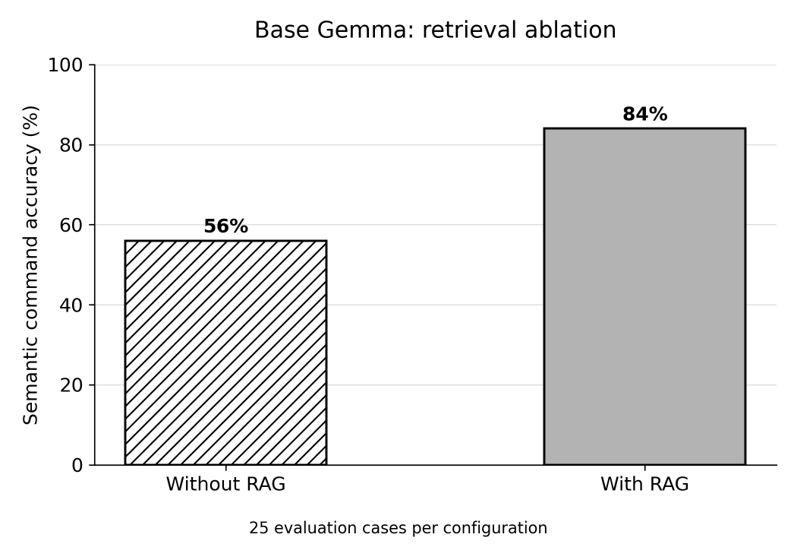
\includegraphics[width=4.39167in,height=3.01425in]{vertopal_80eb40840323498cb949d017d9b2b63a/media/image7.png}

\protect\hypertarget{_Toc242369085}{}{}\emph{Figure 7 Semantic accuracy
without and with RAG in the separate 25-case ablation}

The most useful interpretation is that adaptation improved compliance
with the specialised task and output format, while retrieval supplied
additional documentation context in the smaller base-model experiment.
These findings cannot be combined to claim an independently measured
contribution from every pipeline stage. A factorial comparison using the
same unseen cases would be needed to separate adaptation, retrieval, and
validation effects.

\hypertarget{comparison-with-literature-baselines-and-existing-solutions}{%
\subsection{\texorpdfstring{ Comparison with literature baselines and
existing
solutions}{ Comparison with literature baselines and existing solutions}}\label{comparison-with-literature-baselines-and-existing-solutions}}

PentestGPT, introduced by Deng et al. {[}1{]}, investigates the use of
large language models across penetration-testing tasks. The authors
identify difficulties in maintaining the overall testing context and use
interacting modules to support the workflow. This provides a relevant
comparison for NeuroShell's separation of intent recognition, planning,
execution, and vulnerability analysis.

The present study concentrates on the planning stage. Component 2
receives a structured intent and proposes a command for a supported
tool, with explicit checks on the generated output. Its evaluation
therefore addresses a narrower question than completion of an entire
penetration-testing task. NeuroShell's command exact-match rate cannot
be directly compared with PentestGPT's task-completion results because
the assessment units and experimental conditions differ.

PentestGPT {[}1{]} and NL2Bash {[}3{]} concern related assistance and
translation problems, but use different inputs and evaluation units. RAG
{[}2{]} motivates external knowledge access without establishing
cybersecurity command accuracy. The present results contribute
component-level evidence rather than a claim of superiority over those
systems. The most direct baseline here is the adapter-disabled Gemma
configuration scored with the same strict rule.

\hypertarget{research-contribution}{%
\subsection{Research contribution}\label{research-contribution}}

The main contribution of this work is the development and assessment of
a planning component that connects structured cybersecurity intents to
tool-specific commands. Component 2 brings model adaptation, retrieval,
session context, and validation into a single backend workflow. This
provides a practical implementation of the planning stage within
NeuroShell.

The evaluation contributes evidence about both the model and the
surrounding software. The held-out predictions show how closely the
adapted model reproduced reference commands, while the backend tests
examine whether selected requests and generated outputs received the
expected acceptance or rejection outcome. Assessing these stages
separately makes it possible to identify whether a weakness concerns
generation, input handling, or validation.

The research contribution is the examination of a bounded translation
problem through structured inputs, separate generation configurations,
per-tool results, and explicit validation. It also demonstrates why
reference agreement, tool identity, semantic alignment, and policy
acceptance require distinct interpretation. The findings are useful for
designing a more complete evaluation, including independent reference
review and controlled deployment comparisons

\hypertarget{product-contribution}{%
\subsection{\texorpdfstring{ Product
contribution}{ Product contribution}}\label{product-contribution}}

The evaluation demonstrates why command generation needs to be supported
by explicit checks. A prediction may select the correct tool while
omitting a required argument, changing the target, or introducing an
additional destination. The adapted model's consistent tool selection
therefore provides only one part of the evidence needed to assess a
command.

Within Component 2, command validation checks the generated output
against the structured request. Parsing the command allows target and
port requirements to be assessed in their relevant argument positions.
This distinction matters because a target appearing inside a wordlist
path does not identify the command's destination, and a number used as a
thread count does not satisfy a requested port.

The product contribution is an implemented planning API that connects
intent recognition to command proposal and checking. Modular retrieval,
synthesis, validation, and session management make individual failures
easier to investigate. The resulting component can be integrated with
the surrounding framework, although complete live workflow performance
was not established by the selected tests.

\hypertarget{limitations-and-threats-to-validity}{%
\subsection{Limitations and threats to
validity}\label{limitations-and-threats-to-validity}}

The dataset shaped both what the model learned and how its performance
was measured. Each example linked a structured request to a reference
command, giving the model a consistent task during adaptation. The final
training partition provided reasonably similar representation of Nmap,
Nikto, and Gobuster. However, similar record counts do not necessarily
provide equal coverage of operations, option combinations, or command
complexity.

The distinction between the broader candidate collection and the final
dataset is also important. The candidate collection supplied material
for preparation, while the final partitions contained the examples used
for training, validation, and testing. Keeping these stages separate
makes the development process clearer and allows the reported results to
be interpreted against the data actually used.

Inspection identified reference inconsistencies, including mismatched
targets, incomplete option values, and unclosed quotation marks. These
issues matter because a model may learn an incorrect pattern during
training, while an evaluation may penalise a prediction that corrects an
inaccurate reference. Further dataset improvement should therefore
examine whether each command agrees with its structured input, rather
than checking command text in isolation.

The study assessed command planning for Nmap, Nikto, and Gobuster within
a defined set of structured requests. The results therefore apply to
this scope and do not establish equivalent performance for other
security tools, unsupported operations, or unrestricted natural-language
requests.

Internal validity is limited by the distinct datasets and configurations
used in the direct-model assessment and retrieval ablation. Prompt
changes after inspecting held-out errors can influence later
development; revised configurations need fresh independent evaluation.
The Colab-to-Ollama examples are too few to isolate quantisation or
template effects.

Construct validity is limited by strict textual scoring and imperfect
references. Equivalent syntax can fail exact match, while a matching
malformed reference can still be wrong. The selected pytest pass rate
measures software behaviour under its arrangements. It is not a semantic
model score, a penetration-test completion rate, or proof of
comprehensive safety.

External validity is limited to three tools, the sampled task
distributions, and the tested environments. Similar tool counts do not
imply balanced complex options or rare task families. There was no
formal user trial, concurrency study, final latency benchmark, or
complete licensing clearance. Results therefore should not be
generalised to unrestricted tools, public targets, or production
workloads.

\hypertarget{implications}{%
\subsection{\texorpdfstring{
Implications}{ Implications}}\label{implications}}

For practical use, the findings support a supervised planning workflow
within the assessed scope. Component 2 can propose commands and apply
checks before passing an accepted output to the execution stage. The
results do not establish that generated commands can be used without
review in every environment. Operational permission, tool availability,
and execution outcomes still need to be handled by the wider workflow.

The study also identifies priorities for improvement. These include more
consistent references, better handling of Nmap parameters, and
evaluation of the final model with and without retrieval. The resulting
prototype and recorded assessments provide a basis for investigating
those questions while retaining clear boundaries between command
generation, validation, and execution.

For future development, dataset review and broader semantic assessment
should precede expansion of the supported scope. Nmap requires
particular attention because it produced most non-matches and has
diverse option combinations. Documentation updates should be followed by
retrieval and generation checks. Users should retain an opportunity to
inspect the command and validation result before authorised execution.

\hypertarget{conclusion-and-future-directions}{%
\section{CONCLUSION AND FUTURE
DIRECTIONS}\label{conclusion-and-future-directions}}

\hypertarget{conclusion}{%
\subsection{\texorpdfstring{
Conclusion}{ Conclusion}}\label{conclusion}}

This study developed and evaluated NeuroShell Component 2 as a planning
service for converting structured cybersecurity intents into commands
for Nmap, Nikto, and Gobuster. The adapted model achieved an overall
exact-match rate of 87.54\% on the held-out assessment, while the
selected backend tests supported the implemented validation, safety,
session, and API behaviours.

The findings show the value of combining command generation with
explicit checks. A model can produce a relevant command without
preserving every requirement, and agreement with a reference does not
always establish validity. Structured inputs and command validation
provide a practical means of checking those requirements before an
output reaches the execution stage.

The resulting prototype contributes an implemented planning component to
NeuroShell and a basis for further investigation. Its demonstrated
capabilities remain bounded by the supported tools and assessed
conditions. Improving reference quality, extending semantic evaluation,
and testing the complete workflow would strengthen the evidence for
broader use.

The separate retrieval ablation provides evidence that documentation
context can improve semantic command accuracy under its assessed
conditions, with an observed planning-time cost. The selected software
tests support specific backend behaviours. Taken together, the study
establishes a workable bounded planning prototype and identifies the
evaluation needed before wider use.

\hypertarget{achievement-of-objectives}{%
\subsection{Achievement of objectives}\label{achievement-of-objectives}}

The study implemented the structured-intent workflow, documentation
knowledge base, supported tool selection, model-assisted command
synthesis, validation and safety checks, session handling, and planning
API. These outcomes address the development objectives and provide a
working component boundary for NeuroShell.

The evaluation objective was addressed through paired base/adapted
inference, a separate retrieval comparison, and selected software
verification. Evidence is strongest for strict reference agreement and
tested backend behaviours. A complete final semantic assessment,
aggregate final latency benchmark, stakeholder study, and complete live
workflow evaluation remain unfinished extensions of that objective.

\hypertarget{individual-research-and-product-contributions}{%
\subsection{Individual research and product
contributions}\label{individual-research-and-product-contributions}}

The individual work presented in this thesis focused on Component 2, the
Dynamic Planner and RAG Engine. Its responsibility was to receive
structured cybersecurity intents and produce commands for the supported
tools, providing the planning interface between intent recognition and
execution.

The development contribution included intent interpretation, tool
selection, retrieval-context assembly, and command synthesis. These
functions were connected through a FastAPI backend, with session
management supporting recovery of a previously established target when
required.

The model-development work included preparing structured input--command
examples, adapting the Gemma model, and generating predictions for the
base and adapted configurations. The trained adapter was subsequently
merged with the base model, converted to a quantised GGUF format, and
loaded through Ollama for local inference checks.

\hypertarget{future-directions}{%
\subsection{Future directions}\label{future-directions}}

The first priority is to improve dataset consistency and examine the
remaining command-generation errors. Reference commands should be
reviewed against their structured inputs, with particular attention to
target values, required option arguments, and quotation marks. Further
Nmap examples should address weaknesses identified during error analysis
while maintaining separation between development data and a fresh
assessment set.

Evaluation should also extend beyond exact matching. A documented
semantic assessment could distinguish valid command alternatives from
missing parameters or incorrect operations. Combining this review with
parsing-based checks would provide a clearer account of tool selection,
target preservation, parameter coverage, and overall command
correctness.

A controlled comparison of the final adapted model with and without
retrieval would help establish RAG's additional contribution. The same
inputs, generation settings, and validation procedure should be used in
both configurations. Measuring retrieval and generation separately would
also help explain the relationship between accuracy and response time.

The first priority is to audit inconsistent input--reference pairs while
preserving the originally reported scores. A revised evaluator should
adjudicate supported equivalent syntax and separate formatting
compliance from command meaning. Further experiments should use fresh
held-out cases after any prompt or model changes, measure adaptation and
retrieval under matched conditions, and assess the final local model
against its Colab counterpart.

Subsequent work should evaluate complete authorised execution,
deployment throughput, richer documentation attribution, stakeholder
usability, and maintainable support for additional tool modes. These
steps would connect the present component-level findings to practical
operation without extending claims beyond the available evidence.

\hypertarget{references}{%
\section{References}\label{references}}

\begin{longtable}[]{@{}
  >{\raggedright\arraybackslash}p{(\columnwidth - 2\tabcolsep) * \real{0.0367}}
  >{\raggedright\arraybackslash}p{(\columnwidth - 2\tabcolsep) * \real{0.9633}}@{}}
\toprule()
\begin{minipage}[b]{\linewidth}\raggedright
{[}1{]}
\end{minipage} & \begin{minipage}[b]{\linewidth}\raggedright
G. Deng, Y. Liu, V. Mayoral-Vilches, P. Liu, Y. Li, Y. Xu, T. Zhang, Y.
Liu, M. Pinzger and S. Rass, "PentestGPT: Evaluating and Harnessing
Large Language Models for Automated Penetration Testing," 2024.
\end{minipage} \\
\midrule()
\endhead
{[}2{]} & P. Lewis, E. Perez, A. Piktus, V. Karpukhin, N. Goyal, H.
Küttler, M. Lewis, W.-t. Yih, T. Rocktäschel, S. Riedel and D. Kiela,
"Retrieval-Augmented Generation for Knowledge-Intensive NLP Tasks,"
2020. \\
{[}3{]} & X. V. Lin, C. Wang, L. Zettlemoyer and M. D. Ernst, "NL2Bash:
A Corpus and Semantic Parser for Natural Language Interface to the Linux
Operating System," Miyazaki, Japan, 2018. \\
{[}4{]} & N. Reimers and I. Gurevych, "Sentence-BERT: Sentence
Embeddings using Siamese BERT-Networks," Hong Kong, China, 2019. \\
{[}5{]} & OWASP, "OS Command Injection Defense Cheat Sheet,"
{[}Online{]}. Available:
https://cheatsheetseries.owasp.org/cheatsheets/OS\_Command\_Injection\_Defense\_Cheat\_Sheet.html.
{[}Accessed 7 April 2026{]}. \\
\bottomrule()
\end{longtable}

\hypertarget{appendices}{%
\section{APPENDICES}\label{appendices}}

\hypertarget{appendix-a-research-instruments-or-extended-results}{%
\subsection{Appendix A Research instruments or extended
results}\label{appendix-a-research-instruments-or-extended-results}}

The example below illustrates the structured command-generation
interface. It is an individual generation check, not an additional
held-out accuracy measurement.

\{"intent":"NETWORK\_SCAN","sub\_intent":"specific\_ports\_scan",\\
"target":\{"type":"IP","value":"192.168.1.10"\},\\
"ports":{[}22,80,443{]},"modifiers":{[}"-p 22,80,443"{]},\\
"tool\_hint":"nmap"\}

Recorded Colab and Ollama output: nmap -p 22,80,443 192.168.1.10. This
preserves the requested destination and port selection; it does not show
that the scan executed.

The selected verification run used the following command from the
project root:

python -m pytest tests/integration/test\_plan\_api.py
tests/unit/test\_command\_validator.py
tests/unit/test\_safety\_filter.py
tests/unit/test\_intent\_interpreter.py tests/unit/test\_evaluator.py -v
-\/-tb=short

Run outcome: 42 passed, 1 warning, 71.28 seconds. The selected test run
was recorded on Windows with Python 3.11.9 and pytest 8.2.0. The warning
concerned the multipart import. Prediction artefacts and configuration
requirements are described in Section 3.7.

\hypertarget{appendix-b-academic-integrity-and-ai-use-disclosure}{%
\subsection{Appendix B Academic integrity and AI use
disclosure}\label{appendix-b-academic-integrity-and-ai-use-disclosure}}

Generative AI tools, including ChatGPT and Codex, were used to assist
with drafting, language revision, document organisation, code
troubleshooting, and preparation of this condensed document. AI
assistance was also used to help interpret supplied evaluation records
and format supporting material. These tools were not treated as
independent evidence of system performance.

The reported numerical results are based on the recorded prediction
files, ablation results, and software-test output. Literature claims are
attributed to the listed sources. The candidate remains responsible for
reviewing the final document, verifying the code and analyses, checking
the references, and complying with the applicable academic integrity and
AI-use policy. The disclosure does not replace any separate
institutional declaration or approval requirement.

\end{document}
